\documentclass[a4paper, 11pt]{article}
\usepackage[utf8]{inputenc}
\usepackage[ngerman]{babel}
\usepackage{a4}
\usepackage[a4paper, margin=1in]{geometry}
\usepackage{hyperref}
\usepackage{fancyhdr}
\usepackage{lastpage}
\usepackage{datetime}
\usepackage{graphicx}
\hypersetup{
    bookmarksnumbered,
    colorlinks=true, % set true if you want colored links
    linktoc=all,     % set to all if you want both sections and subsections linked
    linkcolor=blue,  % choose some color if you want links to stand out
    pdftitle={Semesterprojekt Kommunizierende System – Abschlussbericht},
    pdfauthor={David Bachorska, Kevin Cornelius, Rafael Robert Hadamik, Angelina Jellinek,
               Pascal Jochmann, Tom Kieseling, Dennis Ness, Manuel Radatz, Tim Sikatzki,
               Jan Arne Sparka, Kevin Marc Trogant, Lennart Weiß}
}

\renewcommand\labelitemi{\raisebox{0.4ex}{\tiny$\bullet$}}

% Unsere Namen bitte nicht trennen:
\hyphenation{David Bachorska Kevin Cornelius Rafael Robert Hadamik Angelina Jellinek Pascal Jochmann
             Tom Kieseling Dennis Ness Manuel Radatz Tim Sikatzki Jan Arne Sparka Marc Trogant
             Lennart Weiß}

\begin{document}
\sloppy

\pagestyle{fancy}
\fancyhf{}
\renewcommand\headrulewidth{0pt}
\cfoot{\color{red} Rev.: PDF-Dokument erstellt am {\today} um {\currenttime} Uhr \\ % TODO
       (Dieser Hinweis sollte vor der Abgabe noch entfernt werden!)} % TODO

\begin{center}
  \noindent \textbf{\LARGE \center Semesterprojekt \\ „Kommunizierende Systeme“}
  
  \vspace{0.3cm}
  
  \noindent \textbf{\LARGE \center „Lasertag – Nerd Style“}
  
  \vspace{1cm}
  
  \noindent \textbf{\large Wintersemester 2017/2018}
  
  \vspace{0.5cm}
  
  \noindent \textbf{\large Humboldt-Universität zu Berlin \\ Lehrstuhl für Technische Informatik}
  
  \vspace{1cm}
  
  \noindent \textbf{\LARGE Abschlussbericht}
  
  \vspace{2cm}
  \noindent
  \textbf{\large Teilnehmer:} \\
  David Bachorska \\
  Kevin Cornelius \\
  Rafael Robert Hadamik \\
  Angelina Jellinek \\
  Pascal Jochmann \\
  Tom Kieseling \\
  Dennis Ness \\
  Manuel Radatz \\
  Tim Sikatzki \\
  Jan Arne Sparka \\
  Kevin Marc Trogant \\
  Lennart Weiß
\end{center}

\pagebreak

\cfoot{Seite \thepage \hspace{1pt} von \pageref*{LastPage}}

\tableofcontents
\pagebreak

\section{Einleitung}

Das Semesterprojekt „Kommunizierende Systeme” wurde vom Lehrstuhl der Technischen Informatik an der
Humboldt-Universität zu Berlin organisiert und umfasste 12 studentische Teilnehmer.
Betreut wurde es von Stefan Dietzel, Phillipp Schoppmann, Sebastian Henningsen und Björn
Scheuermann.
Das Projekt begann mit dem Wintersemester im Oktober 2017.
Die Zwischenpräsentation fand am 19. Dezember 2017 statt und die Endpräsentation war am
16. Februar 2018.

Das Ziel des Projekts ist es die Studenten zuvor erworbene Kenntnisse aus
Software Engineering und Grundlagen der Programmierung praktisch anwenden zu
lassen. Zur Lösung der gegeben Aufgabe sollen sie ein komplexes System
entwerfen, implementieren, testen und dokumentieren.

Die Aufgabe war die Umsetzung eines eigenen Lasertag mit modifizierten Regeln.
Bei Lasertag handelt es sich um ein Spiel, bei dem mehrere Spieler mit Sendern
in Form von Pistolen und Sensoren ausgestattet werden. Ziel ist es andere
Spieler abzuschießen, um Punkte zu sammeln. Hierbei gibt es verschiedene
Spielmodi, z.B. teambasiert oder jeder gegen jeden. Die besondere Herausforderung
war, dass die Spielregeln so angepasst werden sollten, dass sie einem Peer-to-Peer
Netzwerkprotokoll entsprechen, welches von den Studenten gewählt werden konnten.
Der Entwurf des Systems, dass diese Aufgabe löst, wurde den Studenten völlig
überlassen. Die Spielausrüstung sollte eine physische Form annehmen, sodass
sich die Spieler durch den Raum bewegen können und mit ihrer Umgebung
interagieren können. Es war den Teilnehmern erlaubt Kompromisse zwischen den
originalen Netzwerkprotokollen und der Spielbarkeit zu machen.

Für die Organisation des Projektes wurde Slack verwendet.
Außerdem wurde der vom Informatik-Institut zur Verfügung stehende Gitlab-Server für die
Versionskontrolle genutzt.
Beides wurde durch die Betreuer des Projektes vorgegeben.


\section{Anforderungsanalyse}

Bereits die Forderung, dass das Spiel Lasertag nachgebildet werden soll, hatte weitreichende
Konsequenzen.
Wie im original muss jeder Spieler ein Gerät bekommen, mit dem er andere Spiel abschießen kann und
entsprechend muss ein Abschuss detektiert werden.
Die Spieler sollen dabei möglichst mobil und frei beweglich sein.
Daraus resultiert, dass irgendeine Form von Sender/Empfänger Kombination verwendet werden muss.

Implizit war auch der Spielspaß eine Anforderung.
Dies ist weniger eine technische Anforderung, es verlangt eher, dass die technische Funktionsweise
des Systems nicht nur demonstriert werden kann, sondern auch ausgereift und zuverlässig ist.
Das Spiel sollte so aufbereitet sein, dass jemand mit möglichst wenig Vorkenntnissen ein intuitives
Verständnis entwickeln kann.
Da das Spiel als „Lasertag Nerd Style“ bezeichnet wird, können von der primären Zielgruppe zumindest
grundlegende Vorkenntnisse zu Netzwerkpotokollen erwartet werden. Dennoch muss das P2P-Protokoll der
Wahl in die Form eines spielgerechten Regelwerks transformiert werden.

Es wurden keine genaueren Anforderungen an die Spielgeräte gestellt, daher kann sich das Team eine
beliebige Architektur aussuchen, die das Spiel unterstützt.
Um den Spielspaß zu gewärleisten, muss jedoch die Übertragung von Treffern zuverlässig sein und die
Geräte sollten möglichst handlich und leicht zu bedienen sein.
Die Spieler brauchen insbesondere eine Möglichkeit Feedback darüber zu erlangen, ob sie einen
Spieler getroffen haben und wie das Spiel derzeit verläuft. Auch gilt, dass eine möglichst bequeme
Lösung für den Spieler den Spaß unterstützt.

Aus den Anforderungen für Bequemlichkeit ergibt sich, dass drahtlose Kommunikationsmethoden
verwendendet werden sollten und die Spielgeräte über Akkumulatoren betrieben werden sollten.
Die Sensoren sollten entweder am Spielgerät befestigt sein, oder es sollte möglichst einfach am
Körper anbringbar und robust sein.

Da drahtlose Kommunikation verwendet wird und das Spiel möglichst reibungslos ablaufen soll, muss
insbesondere bedacht werden, dass es zu Störungen kommen könnte und somit Informationen verloren
gehen.
Es ist also notwendig, dass die Geräte von einem unzuverlässigen Übertragungskanal ausgehen und mit
daraus resultierenden Problemen umgehen können.
Es ist außerdem zu beachten, dass es zu Schwierigkeiten mit konkurrierenden Prozessen kommen kann,
weil z.B. Signal X schneller als Signal Y empfangen wurde, obwohl Signal Y früher abgeschickt wurde.


\section{Systemarchitektur}

In diesem Abschnitt wird das geplante System beschrieben, mit dem die Gruppe die Anforderungen
erfüllen möchte.
Die \cref{fig:architecture} stellt die Systemarchitektur dar.

\begin{figure}[h]
  \centering
  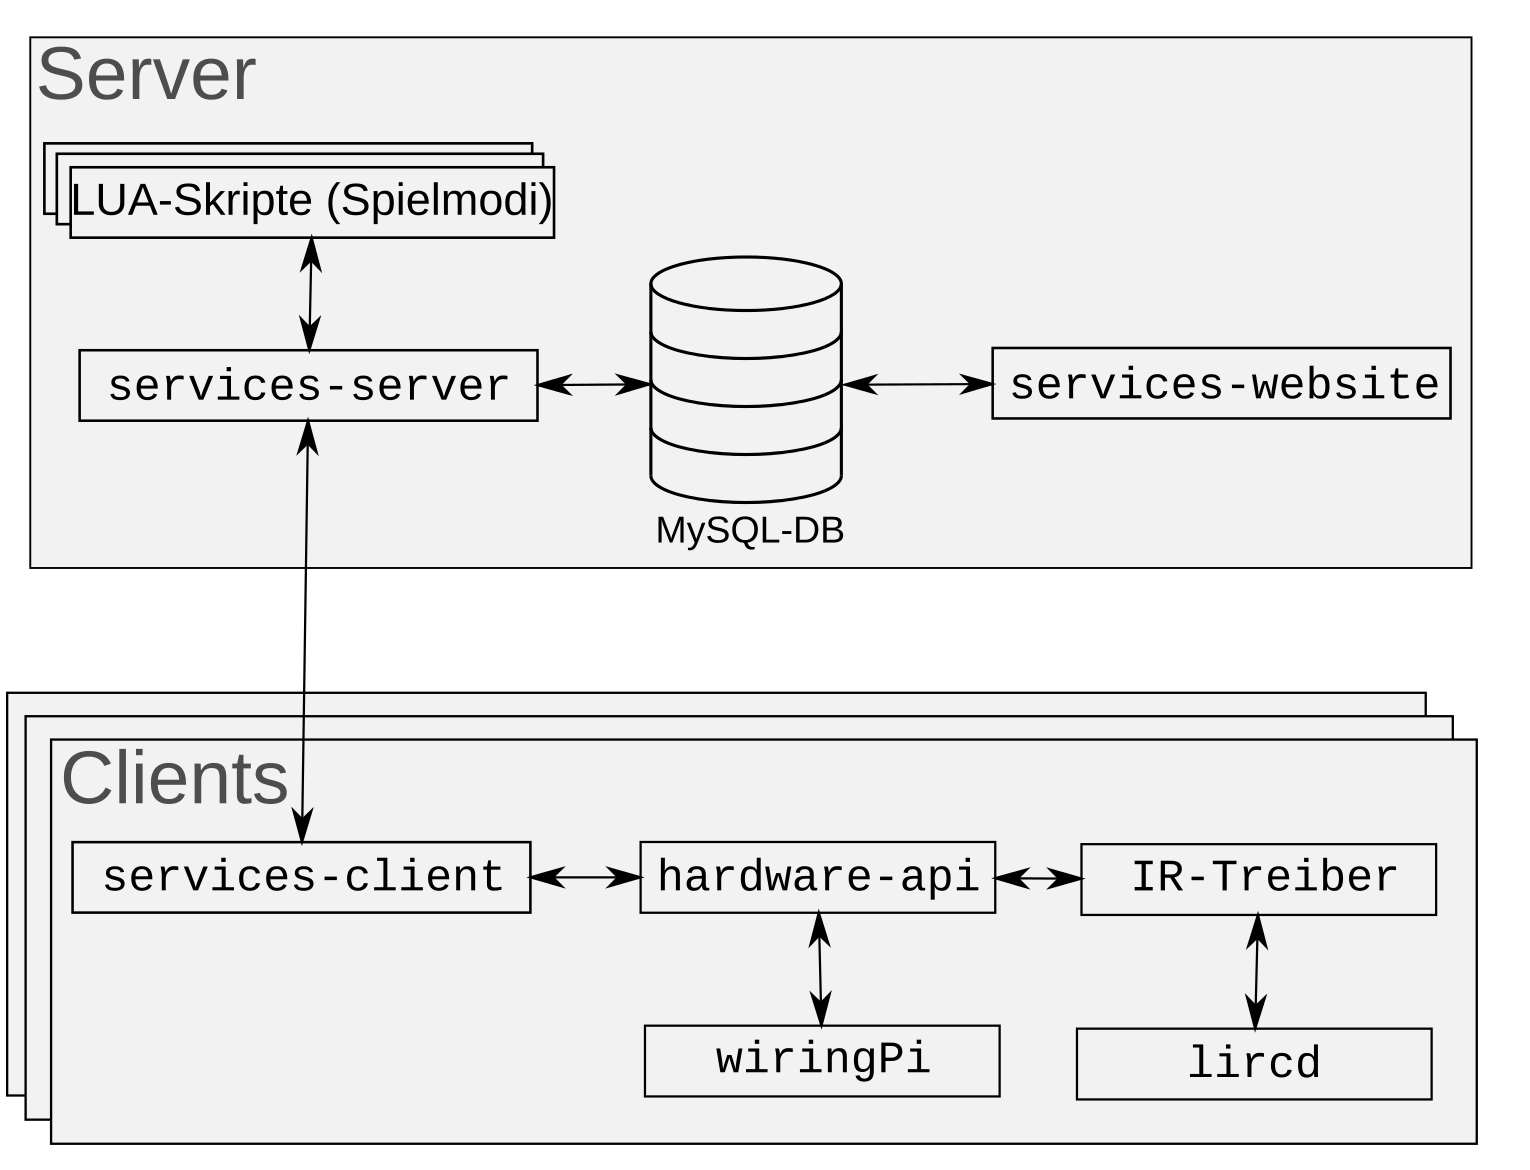
\includegraphics[width=0.7\textwidth,keepaspectratio]
                  {./030-systemarchitektur/architecture.png}
  \caption{Ein Überblick über die Systemarchitektur}
  \label{fig:architecture}
\end{figure}

\subsection{Die Spielgeräte}

Wie oben bereits beschrieben, war für das Nachbilden von Lasertag eine drahtlose Übertragungsmethode
notwendig, die möglichst zuverlässig ist.
Im realen Lasertag wird dafür Infrarot verwendet und es werden LEDs benutzt, um den Abschuss
darzustellen.
Auch in diesem Projekt fiel die Wahl auf Infrarot.
Es ist im Gegensatz zu Laser nicht schädlich für die Augen und es können über eine größere Distanz
zielgerichtet gesendet werden.
Es gibt kostengünstige Komponenten wie LEDs und Sensoren, sowie Open Source Treiber für die
Modellierung für Daten.
Es reicht nicht aus, einfach nur zu erkennen, dass man getroffen wurde, weil es für die Spielregeln
notwendig ist zu wissen, von welchem Spieler der Schuss kam.
Diese Notwendigkeit ergibt sich daraus, das zwei Systeme die über das Netzwerk kommunizieren, dazu
in der Lage sein müssen sich eindeutig zu identifizieren.
Daher war es sehr nützlich, dass über Infrarot Daten versendet werden können, wie zum Beispiel bei
Fernbedienungen.

Die gegenseitige Identifizierung wurde so gelöst, dass das Spielgerät eines Spielers beim Abschuss
eine ID versendet.
Wenn der Sensor eines Spielers diese ID empfängt, weiß das Gerät von wem der Schuss kam und es weiß
ebenso seine eigene ID.
Daher hat es eine Information der Form: Spieler X hat Spieler Y getroffen.

Als Gerät fiel die Wahl auf den Raspberry Pi Model Zero W. Die Entscheidung wurde getroffen, weil
ein leichter, stromsparender Computer benötigt wurde, der freiprogrammierbar ist und mit
Infrarotkomponenten erweitert werden kann.
Für den kabellosen Betrieb werden Powerbanks verwendet, um die Geräte mit Strom zu versorgen.

Als zu spielendes Netzwerkprotokoll haben wir eine vereinfachte Version von Bittorrent gewählt.
Diese Wahl fiel unter anderem, da dieses Original auch in der Realität spielerische Elemente bietet.
So gibt es im Netzwerk etwa Teilnehmer, die möglichst viel Datenvolumen von anderen beziehen wollen,
ohne selber eine entsprechende Upload-Bandbreite anzubieten.
Dieses Element der Fairness sollte eine zentrale Komponente im Spiel sein.

Tatsächlich wurden mehrere Spielmodi implementiert.
Dies geschah aus verschiedenen Gründen:
\begin{enumerate}
  \item
    Es zwang uns eine modulare Architektur zu errichten, die völlig unabhängig vom gewählten
    Spielmodus funktioniert.
    Dadurch habe wir eine garantierte Flexibiltät, Änderungen an Spielmodi vornehmen zu können.
  \item
    Die Spielmodi haben eine unterschiedliche Reichhaltigkeit an Funktionen.
    Dies ist nützlich für das Debugging, weil somit gezielt Features getestet und gewisse
    Rahmenbedingungen je nach Spielmodus vernachlässigt werden können.
\end{enumerate}


\subsection{Netzwerkarchitektur}
\label{sec:architektur-netzwerkarchitektur}

Informationen über Abschüsse müssen eine entsprechende Auswirkung auf den Spielstand haben.
Eine Option dafür wäre, dieselbe Applikation auf jedem Gerät zu installieren und ein P2P-Netzwerk zu
errichten, in dem sich die Geräte konstant über den gegenwärtigen Spielstand austauschen.
Daraus resultiert jedoch ein sehr kompliziertes Protokoll zur Synchronisierung, insbesondere weil
ein Gerät mitten im Spiel die Verbindung verlieren könnte.
Stattdessen wurde eine simplere Client-Server-Architektur gewählt, in der Clients lediglich
Informationen sammeln und diese an den Server weiterreichen.
Der Server wertet sie aus und gibt Informationen über den Spielstand an die Clients zurück.
Durch diese Architektur werden viele potenzielle Logikfehler, die sich durch konkurrente Nachrichten
ergeben, eliminiert.

Die Clients und der Server verwenden zur Kommunikation WLAN. Dies ist die naheliegendste Lösung, da
die Technik zuverlässig ist und Verbindungsprobleme größtenteils durch den TCP/IP-Stack des
Betriebssystems gelöst werden.
Um ein weitaufspannendes Feld zu errichten, wäre es notwendig, mehrere Access Points (AP) zu
errichten, die sich mit Roaming austauschen.
Es wurde allerdings entschieden, dass dies den Rahmen des Projekts sprengen würde und es wurde der
Einfachheit halber entschieden, den Server auch gleichzeitig als AP einzusetzen, womit theoretisch
ein Spielfeld unterstützt wird, dass mehrere Räume umspannt.


\subsection{Das Spiel}
\label{sec:architektur-spiel}

Zuvor wurde die grundlegende Infrastruktur beschrieben, mit der Informationen über Abschüsse
ausgetauscht werden können.
Das allein reicht für das Spiel noch nicht aus, weil die Spieler eine Möglichkeit brauchen, eine
Übersicht über den Spielstand zu bekommen.
Dafür gibt es zwei Ansätze, die verfolgt wurden:
\begin{itemize}
  \item
    eine Anzeige auf jedem Gerät über den Status des Spielers und
  \item
    eine Anzeige für den Server über den aktuellen Spielstand.
\end{itemize}
Die Anzeige für die Spielgeräte wurde mit LEDs realisiert, die mit verschiedenen Farben anzeigen, ob
ein anderer Spieler getroffen wurde, ob man unverwandbar ist, etc.
Dies ist eine preiswerte Möglichkeit, die durch die GPIO-Anschlüsse der Raspberry Pis unterstützt
wird.
Mehr zu den LEDs ist im \cref{sec:leds} zu finden.

Die Anzeige des Servers wurde mit einer Webseite umgesetzt, die tabellarisch das Scoreboard anzeigt.
Die Webseite soll auf einem oder mehreren Bildschirmen dargestellt werden, die auf das gesammte
Spielfeld verteilt werden.

In dieser Entscheidung spiegelt sich wider, dass Spieler regelmäßig erfahren wollen, ob sie noch im
Spiel sind oder ob sie einen anderen Spieler getroffen haben.
Daher muss es eine Möglichkeit geben, die entsprechende Anzeige sehr schnell und einfach zu
überprüfen.
Der aktuelle Spielstand muss seltener angesehen werden, weshalb es in Ordnung ist, wenn der Spieler
einige Sekunden braucht, um auf die Webseite zu schauen.

Letztendlich muss auch auf Fairness geachtet werden.
Daher ist es wichtig, dass die Fähigkeit, andere Spieler abzuschießen, limitiert ist.
Dies muss auf mehrere Weisen geschehen:
\begin{enumerate}
  \item
    Die Streuung von Abschüssen muss eingeschränkt sein.
    Dies wurde gelöst, indem Strohhalme über die IR-LEDs gestülpt wurden, die das Aussenden des
    Signals in eine bestimmte Richtung lenken.
  \item
    Damit ein Spieler nicht mehrmals hintereinander getroffen werden kann, gibt es bei vielen
    Spielmodi eine kurze Unverwundbarkeitszeit, nachdem ein Spieler getroffen wurde.
    In dieser Zeit hat der Getroffene die Möglichkeit, sich so zu positionieren, dass er nicht
    erneut getroffen wird.
\end{enumerate}


\subsection{Die Spielmodi}

Es wurde entschieden, dass die Spielelogik möglichst vom Backend getrennt sein soll.
Deswegen wurde sie in Form von LUA-Skripts gekapselt und wird vom Server eingebunden.
Die Schnittstelle zwischen diesen beiden Komponenten ist ein Informationsaustausch.
Der Server gibt Spielparameter und Abschussinformationen an LUA weiter und die Spielelogik gibt die
resultieren Auswirkung auf den Spielstand zurück, damit dieser auf der Website und den Geräten
angezeigt werden kann.

Als zu spielendes Netzwerkprotokoll haben wir eine vereinfachte Version von Bittorrent gewählt.
Diese Wahl fiel unter anderem, da dieses Original auch in der Realität spielerische Elemente bietet.
So gibt es im Netzwerk etwa Teilnehmer, die möglichst viel Datenvolumen von anderen beziehen wollen,
ohne selber eine entsprechende Upload-Bandbreite anzubieten.
Dieses Element der Fairness sollte eine zentrale Komponente im Spiel sein.

Tatsächlich wurden mehrere Spielmodi implementiert.
Dies geschah aus verschiedenen Gründen:
\begin{enumerate}
  \item
    Es zwang uns eine modulare Architektur zu errichten, die völlig unabhängig vom gewählten
    Spielmodus funktioniert.
    Dadurch habe wir eine garantierte Flexibiltät, Änderungen an Spielmodi vornehmen zu können.
  \item
    Die Spielmodi haben eine unterschiedliche Reichhaltigkeit an Funktionen.
    Dies ist nützlich für das Debugging, weil somit gezielt Features getestet und gewisse
    Rahmenbedingungen je nach Spielmodus vernachlässigt werden können.
\end{enumerate}



\section{Komponenten}

Aus der Anforderungsanalyse ergeben sich drei abstrakte Komponenten:
\begin{enumerate}
  \item
    die Spielgeräte und hardwarebasierte Infrastruktur
  \item
    Kommunikation der Spielgeräte und softwareseitige Infrastruktur
  \item
    das Entwerfen eines Spielkonzepts und die Umsetzung in Software
\end{enumerate}
Es handelt sich hierbei um ein System mit mehreren Schichten, wobei jede Schicht Dienste für die
darüberliegende Schicht anbietet.
Man kann feststellen, dass die Trennung der Komponenten nicht sauber ist.
Es ist zum Beispiel unklar, wo die hardwarebasierte Infrastruktur in die softwarebasierte übergeht,
etwa bei Netzwerkprotokollen.

Bei der Arbeit am Semesterprojekt haben wir den Komponenten entsprechend die Teilnehmer in drei
Gruppen eingeteilt, welche abgekürzt als „\hyperref[sec:hardware]{Hardware}“,
„\hyperref[services]{Services}“ und „\hyperref[sec:spiellogik]{Spiellogik}“ bezeichnet werden.
In den folgenden Abschnitten werden die jeweiligen Gruppenmitglieder aufgezählt und die
Arbeitsergebnisse derselben erläutert.

\subsection{Hardware}
\label{sec:hardware}

Mitglieder und Aufgaben:
\begin{itemize}
  \item
    Kevin Cornelius (Schaltungen, Spielgeräte)
  \item
    Lennart Weiß (Installation, Betriebssystemkonfiguration)
  \item
    Manuel Radatz (API, Spielanzeige)
  \item
    Rafael Robert Hadamik (Infrarottreiber, Spielgeräte)
\end{itemize}

\subsubsection{Spielgerät}
\label{sec:hardware-spielgeraet}

Die Spielgeräte wurden von Kevin Cornelius entworfen und von ihm und Rafael Hadamik gebaut.
Das Spielgerät, in \cref{fig:Bild1Hardware} zu sehen und nachfolgend genannt „Tagger“, ist eine Infrarot-Pistole inklusive Empfänger. Die einzelnen Spieler benötigen beim Spielen des Lasertags nur den „Tagger“ und keine Weste. Deshalb bleiben sie voll beweglich und es erhöht gleichzeitig den Schwierigkeitsgrad. \\
Bei der Wahl der Materialien musste man vor allem das Budget, die Stabilität und die Handhabung berücksichtigen, damit ein vernünftiges Spiel enstehen kann. Daraus folgt der grundlegende Aufbau des „Taggers“:
\begin{enumerate}
	\item Die Schaltungen wurden mit einzelnen Komponenten, Jumper-Kabeln und Lochrasterplatten gesteckt und gelötet.
	\item Die Infrarot-LED wird durch ein Aluminiumrohr gerichtet, damit ein gebündelter Infrarot-Strahl entsteht und die natürliche Streuung eines Infrarot-Signals nicht das Spielen erschwert.
	\item Als Rechensystem wurde ein Raspberry Pi Zero W benutzt, dieser  hat die oben beschriebenen Anforderungen am Besten erfüllt.
	\item Der Akkumulator konnte aufgrund des geringen Stromverbrauches mit geringer Kapazität, kleinen Abmessungen und geringem Preis gewählt werden.
	\item Das Gehäuse des „Taggers“ wurde mit Acrylglas und der Benutzung geeigneter Werkzeuge hergestellt. Acrylglas ist sehr bruchsicher und leicht, was beides sehr geeignete Eigenschaften für dieses Gehäuse sind.
\end{enumerate}
\begin{figure}[h]
	\centering
		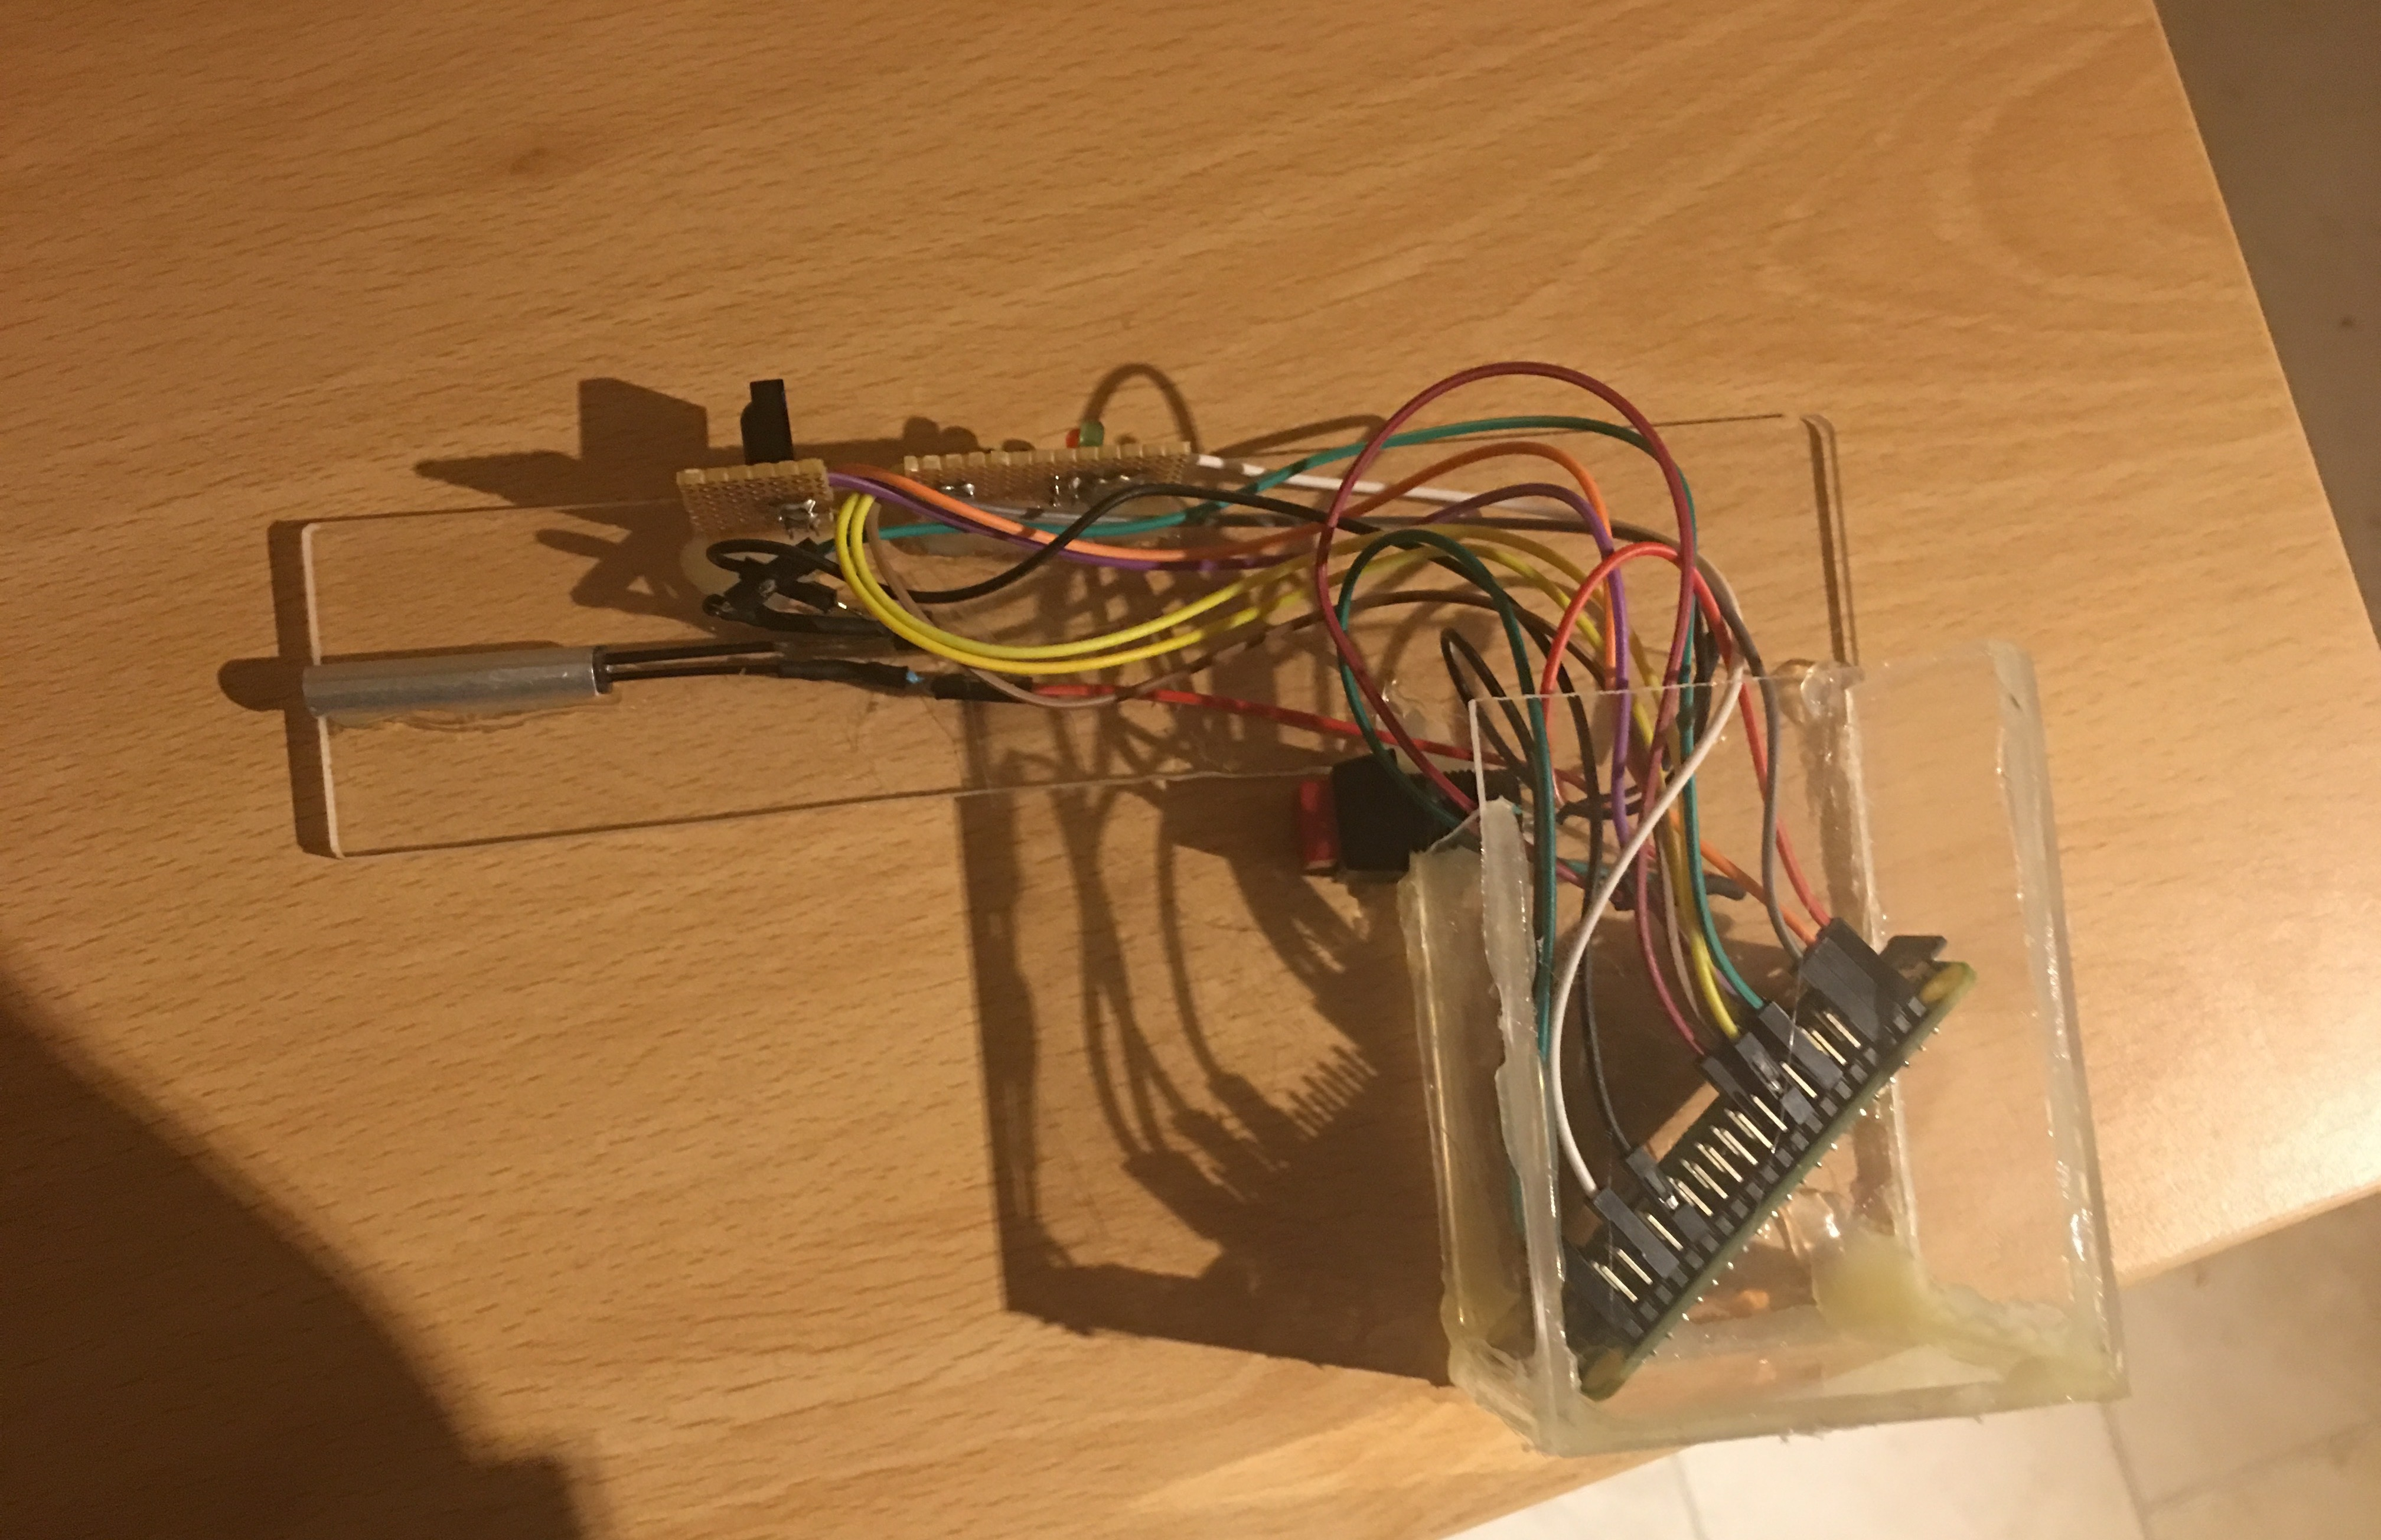
\includegraphics[width=0.7 \textwidth]{./040-komponenten/010-hardware/tagger.jpg}
	\caption{Das Spielgerät}
	\label{fig:Bild1Hardware}
\end{figure}



\input{./040-komponenten/010-hardware/schaltungen}

\subsubsection{Betriebssysteminstallation}

Dieser Abschnitt erläutert, wie die Grundinstallation auf den Spielgeräten und dem Server
vorgenommen wird.
Für diese Aufgabe war Lennart Weiß verantwortlich.

Der Server ist ein Raspberry Pi Model B+.
Er hat zwei physikalische Netzwerkinterfaces: WLAN und Ethernet.
Aufgrund der geringen Größe lässt er sich leicht überall hin transportieren.
Für ein Spiel benötigt er lediglich eine Stromversorgung, um als internetfähiger Access Point zu
dienen braucht darüber hinaus einen Ethernet Uplink, über dem er per DHCP eine IP Adresse beziehen
kann und Internetzugang hat.
Zum Debugging sind darüber hinaus Bildschirm und Tastatur nützlich.

Auf dem Server ist Raspbian Lite installiert.
Das Gerät lässt sich auch durch einen beliebigen anderen PC austauschen, dass besagte
Netzwerkschnittstellen besitzt und auf dem Debian installiert werden kann (was den meisten gängigen
Prozessorarchitekturen möglich ist).
Raspbian wurde vor allem wegen seiner weiten Verbreitung und Stabilität gewählt.
Für Probleme bei der Serverinstallation kann im Regelfall eine Suche in Debianforen und ähnlichem
eine Lösung gefunden und auf Raspbian übertragen werden.

Auf dem Server ist ein Puppetmaster eingerichtet.
Damit kann genau festgelegt werden, welche Software auf die Clients verteilt werden soll und die
Installation kann automatisiert werden.
Für jeden Client muss auf dem Server ein Zertifikat signiert werden, dieser manuelle Schritt wird
jedoch nur einmal bei der Erstinstallation des Client vorgenommen.
Für die möglichst schnelle Installation der Spielgeräte wurde ein Image mit Raspbian vorbereitet, in
dem eine deutsche Lokalisierung mit englischer Sprache eingestellt wurde und ein Puppet Client
installiert ist.
Außerdem wurde die WLAN SSID und das Passwort eingerichtet und der Client verbindet sich nach dem
Boot Vorgang automatisch per wpa\_supplicant mit dem Server.
Um den Kopiervorgang zu beschleunigen, wurde das Image auf die minimale Größe (ca. 2G) gehalten.
Dadurch kann das Image in wenigen Minuten auf eine SD Karte geschrieben und in den neuen Raspberry
Pi eingesetzt werden.
Außerdem kann die SD Karte eine beliebige Größe haben.

Um den Installationsvorgang zu beenden, muss auf man sich per SSH auf dem Client einloggen.
Per raspi-config wird das Filesystem auf die maximale Größe eingestellt und der Hostname
eingestellt.
Dieser ist ‚\texttt{client-x}‘, wobei \texttt{x} die Client ID bezeichnet, welche vorher eindeutig
an jedes Gerät vergeben wird.
Die Geräte sind entsprechend beschriftet, damit sie identifiziert werden können.
Schließlich werden mit Puppet alle benötigten Komponenten installiert und der Client ist
einsatzbereit.



\subsubsection{Netzwerkkonfiguration}

Dieser Abschnitt erläutert die Netzwerkinfrastruktur des Projekts.
Für diese Aufgabe war Lennart Weiß verantwortlich.

Die Spielgeräte kommunizieren miteinander über ein WLAN Netzwerk. Die
Netzwerkkonfiguration wird zentral über den Server geregelt. Verglichen mit
einem P2P-Netzwerk oder Infrastruktur Wifi mit Roaming ist der Administrations-
aufwand relativ gering und gleichzeitig sind die Verbindungen stabil, solange
sich die Geräte nah am Server aufhalten.

Um den Server als Access Point zu verwenden wurde das Program hostapd verwendet,
welches den Onboard Wifi Chip des Raspberry Pi verwendet, um ein Netzwerk
aufzuspannen. Diese Chips sind eigentlich dafür gedacht, dass der Raspberry Pi
selber als Client dient und sich zu einem anderen Netzwerk verbindet. Für lange
Distanz und hohe Stabilität wäre eine externe Netzwerkkarte mit Antenne
womöglich besser geeignet. Dennoch hat sich in praktischen Versuchen gezeigt,
dass sich das Coding Tag Netz über mehrere Räume hinweg stabil verwenden lässt
und ist somit für kleine Spielfelder und technische Demonstrationen vollkommen
ausreichend.

Mit dem zuvor beschriebenen Netzwerk allein wäre es bereits möglich gewesen
das Projekt zu realisieren. Allerdings wurden noch weitere Funktionalitäten
hinzugefügt, um zum einen die Projektarchitektur zu verbessern und zum anderen
einen gewissen Komfort zu bieten. Die grundsätzliche Anforderung, die wir uns
selber gestellt haben, war, dass die Clients sich lediglich mit dem Netzwerk
verbinden sollen und die gesamte restliche Konfiguration auf dem Server 
stattfinden soll. Dies reduziert die Notwendigkeit für doppelte Arbeit, da der
Server nur einmal installiert werden muss, Clients jedoch öfter. Außerdem hat
der Server mehr Kontrolle und bei Fehlverhalten liegt die Ursache meistens beim
ihm.

Um DHCP und DNS anbieten zu können, wurde dnsmasq installiert. IP-Adressen
werden aus dem frei wählbarem Adressraum 10.0.0.0/8 gewählt. Dem Server wurde
10.0.0.1 vergeben, die Clients erhalten Adressen aus dem Bereich 10.0.1.1 bis
10.0.1.254. Dies beschränkt die maximale Anzahl an Geräten die am Spiel
teilnehmen können, allerdings wurde anfangs mit einer Spielerzahl von ca.
einem Dutzend gerechnet und falls notwendig lässt sich der Adressbereich einfach
vergrößern. Anfangs gab es im Projekt ein statisches Mapping zwischen der
Client ID und der IP Adresse, z.B. wurde client-2 immer 10.0.1.2 vergeben.
Dies ist nützlich, weil in Logs und dergleichen aus der IP Adresse sofort auf
den Client geschlossen werden kann. Allerdings erwies sich dieses Mapping nicht
als nützlich, weil in der Software nur mit Hostnames gearbeitet wird. Außerdem
war es notwendig, dass die Mappings von ID zu MAC Adressen in einer Datei
gespeichert werden, was zusätzlichen Aufwand bei der Installation bedeutete.
Da die statischen Adressen nur wenig zusätzlichen Nutzen bringen werden nun
Clients beliebige Adressen aus dem verfügbarem Pool zugewiesen.

Im gesamten Projekt wird niemals direkt mit IP Adressen gearbeitet, auf
Software Ebene sprechen sich die Geräte gegenseitig mit Hostnames an. Damit
können in der Netzwerkschicht Änderungen vorgenommen werden, ohne dass die
Software entsprechend geändert werden muss. Die Hostnames werden direkt auf
den Clients gesetzt, dadurch ist bei der Installation eines neuen Gerätes keine
Änderung am Server notwendig. Damit sich die Geräte gegenseitig mit Hostnames
ansprechen können, beantwortet der Server DNS Anfragen und gibt die
erforderliche IP Adresse zurück. Diese kennt der Server, weil er selbst als
DHCP Server jene Adressen vergeben hat.

Die Geräte, sowie der Server, sollten in der Lage sein sich mit dem Internet
zu verbinden, um Pakete herunterladen zu können. Diese Verbindung soll jedoch
optional sein und für keine Komponente im Projekt wird eine Internetverbindung
verwendet, sie ist lediglich im Installationsprozess notwendig. Hierfür wird
die Ethernet Schnittstelle (eth0) des Servers mit einem Uplink verbunden, über
den per DHCP eine IP Adresse und Zugang zum Internet bezogen werden kann. Die
Routingregeln sind so eingestellt, dass eth0 die Default Schnittstelle ist und
lediglich Pakete im 10.0.0.0/8 Netzwerk über die WLAN Schnittstelle gesendet
werden. Damit auch die Client Geräte Internetzugang haben, ist auf dem Server
IP Forwarding aktiviert und es wird NAT mit einfachem Port Forwarding verwendet,
damit Pakete von außen die Clients erreichen, ohne dass die Clients selber eine
IP Adresse in dem Netz brauchen. Damit auch Namen außerhalb des eigenen Netzes
auflösen können, wird der Server als DNS Cache verwendet, der einen externen
Nameserver (8.8.8.8) verwendet für Ziele die er nicht kennt.


\subsubsection{Installation des Projekts}
\label{sec:installation-des-projekts}

Dieser Abschnitt erläutert, wie die einzelnen Komponenten des Projekts auf die
Geräte verteilt werden. Für diese Aufgabe war Lennart Weiß verantwortlich.

In den vorherigen Abschnitten wurde die Basis für unser Projekt vorgestellt.
Allerdings blieb offen, wie die verschiedenen Komponenten verteilt werden.
Dafür gibt es grundsätzlich zwei Anforderungen: Zum einen muss festgelegt
werden, aus welchen Komponenten das System besteht und welche Installationsschritte
notwendig sind. Zum anderen muss ein Prozess definiert werden, mit dem
die Installation automatisiert vollzogen wird. Letzterer Schritt ist aus
verschiedenen Gründen wichtig. So können durch einen automatisierten
Prozess Flüchtigkeitsfehler ausgeschlossen werden. Aber vor allem die Geschwindigkeit,
mit der simultan die neueste Version unserer Software auf alle Geräte verteilt
werden kann, ist ausschlaggebend. Müsste dies manuell gemacht werden, wäre es
unmöglich, an einem Tag mehrere verschiedenen Versionen auf den Geräten zu
testen, weil nach jeder Änderung die Software neu verteilt werden muss.

Die Systemkomponenten wurden bereits beschrieben. Im folgenden Abschnitt wird
erklärt, wie diese auf welchem System installiert werden. Zuerst müssen externe
Voraussetzungen erfüllt werden. Auf dem Server werden diverse MySQL-Pakete
installiert und auf dem Client einige Lirc-Pakete. Die lirc-Konfiguration muss
angepasst werden und es müssen beim Systemstart zusätzliche Treiber geladen
werden. Die dafür notwendigen Konfigurationsdateien befinden sich im Hardware-Repository.
Die verschiedenen Spielmodi sind LUA-Dateien und befinden sich
im Spielmodus-Repository. Sie sollen auf dem Server nach 
\texttt{/var/lib/spielmodi} kopiert werden. Die Webseite besteht aus einer
Python-Datei und einigen HTML-Seiten. Diese befinden sich in einem Ordner im
Services-Repository und sollen auf dem Server nach 
\texttt{/usr/bin/services-website} kopiert werden. Außerdem müssen mit Pip
einige zusätzliche Pakete installiert werden. Die restlichen Dateien
müssen noch zuvor kompiliert werden. Die daraus resultierenden Binaries 
\texttt{services-client} und \texttt{hardware-api} sollen auf den Client nach
\texttt{/usr/bin} kopiert werden und ebenso \texttt{services-server} auf
den Server. Die Shared Library \texttt{libservices-common.so} wird auf allen
Geräten nach \texttt{/usr/lib} verschoben und auf dem Server wird zusätzlich
\texttt{/usr/libmysqlclient.so.18} in dasselbe Verzeichnis kopiert.

Da nun festgelegt ist was installiert werden soll, erläutern wir den
automatisierten Prozess, um dies zu bewerkstelligen. Auf dem Server befindet
sich ein Skript, das jedes Mal ausgeführt wird, wenn die neueste Version des
Projekts verteilt werden soll. Bevor das Skript aufgerufen wird, muss die
gewünschte Version von Gitlab heruntergeladen werden. Wenn es in der neusten
Version einen schwerwiegenden Fehler gibt, ist es somit möglich auf eine
funktionierende umzusteigen. Als nächstes werden diverse Makefiles aufgerufen,
um die Binaries zu kompilieren. Danach werden die Dateien, die auf dem Server
installiert werden sollen, direkt in die entsprechenden Verzeichnisse kopiert.

Der Installationsprozess für die Clients wird mit einem Orchestrationstool
names Puppet organisiert. Der Server ist der Puppetmaster und in einem
speziellen Ordner befindet sich die Beschreibung des erwünschten Systemzustands
der Client sowie die Dateien, die dafür auf den Client kopiert werden müssen.
Der Vorteil in der Verwendung dieses Werkzeugs ist, dass der erwünschte
Systemzustand der Clients in Gitlab dokumentiert und unter Versionskontrolle
ist. Außerdem kümmert sich nun Puppet im Hintergrund um die Installation und
ist in der Lage, im Falle eines Fehlschlags den bisherigen Installationsprozess
rückgängig zu machen und das System in den bisherigen Zustand zu bringen. Das
Installationsskript auf den Server kopiert automatisch alle für die Clients
benötigten Dateien in das Puppet-Verzeichnis. Die Clients werden nun entweder
innerhalb der nächsten halben Stunde auf die neueste Version umsteigen, oder
der Update-Prozess kann manuell sofort gestartet werden.

Nun müssen die Applikationen noch gestartet und Abhängigkeiten gelöst werden.
Dafür wurde Systemd verwendet. Es ist die Systemstartlösung von Raspbian und
definiert, welche Applikationen in welcher Reihenfolge gestartet werden. Um
den Spielstart zu vereinfachen, sollen die Coding-Tag-Programme bereits starten,
wenn die Geräte mit Strom versorgt werden. Für jedes Programm gibt es eine
Systemd-Unit, die bei jedem Systemstart ausgeführt wird. Damit kann die
richtige Reihenfolge durch Abhängigkeiten definiert werden. Auf dem Server
sind die Webseite und der Services-Server von MySQL abhängig. Auf dem Client
hängt der Services-Client von der Hardware-API ab und diese wiederum von Lirc.
Sollte ein Service abstürzen, können die Fehlermeldungen im Systemlog
nachgelesen werden. Außerdem lassen sich die Programme über \texttt{systemctl}
komfortabel starten oder stoppen.



\subsubsection{IR-Treiber}

Um die einzelnen Spieler zu unterscheiden, war es notwendig, dass sie unterschiedliche
Informationen aussenden, um sie eindeutig im Spielkontext zu identifizieren.
Wir hatten drei verschiedene Ideen, wie man diese Informationen modellieren kann, um sie schnell und 
korrekt zu übertragen.
Dabei war die Grundlage, dass jede gesendete Information in eine eindeutige Abfolge von 2
verschiedenen Zuständen – im Folgenden als Zustand 0 (kurz: 0) bzw. Zustand 1 (kurz: 1)
bezeichnet – übersetzt wird und dann diese Abfolge von Zuständen gesendet wird.
Diese Abfolge von Zuständen musste ebenfalls modelliert werden, um das Gebot der Korrektheit zu
erfüllen, da ein einfaches Absenden der Information – mit Signal an $= 1$ und Signal aus $= 0$ –
sehr rauschanfällig wäre.
Des Weiteren wollten wir auf selbstkorrigierende Codes verzichten, um eine möglichst schnelle und
genaue Treffererkennung zu schaffen, und um zu verhindern, dass wenn zwei Spieler nahezu
gleichzeitig schießen, der Spieler, der zuerst schießt, den Treffer nicht gewertet bekommt, da sein
Schuss erst korrigiert werden musste, wohingegen der Schuss des langsameren Spielers zuerst gewertet
wird, da sein Schuss keine Korrektur hatte.
Dazu hatten wir folgende drei Ideen, wie man diese Modulation umsetzen könnte:
\begin{enumerate}
  \item
    Man gibt Zustand 1 und Zustand 0 unterschiedliche Längen von einem Signal mit festen Pausen
    dazwischen.
  \item
	Man modeliert die Zustände über Signalflanken.
  \item
	Man gibt beiden Zuständen die gleiche Signalzeit, aber unterschiedliche Pausen zwischen den
	einzelnen Signalen.
\end{enumerate}

\paragraph{Idee 1}
Der Vorteil der ersten Idee ist, dass sie sehr simpel zu implementieren ist.
Der Nachteil ist jedoch, dass sie von den drei Ideen am stärksten rauschanfällig ist und somit die
geringste Reichweite bietet.

\paragraph{Idee 2}
Die Vorteile hier bestehen darin, dass sie sehr einfach zu implementieren wäre, wenn man den Treiber
von Grund auf selbst schreibt, und dass sie die schnellste Übertragung von allen bietet.
Der größte Nachteil besteht jedoch darin, dass diese Idee selbst sehr rauschanfällig ist, da Flanken
in der Theorie überspielt werden könnten.

\paragraph{Idee 3}
Der Vorteil besteht hier darin, dass die geringste Rauschanfälligkeit besteht, da man – mit genügend
großen Unterschieden zwischen den Pausen bei den beiden Zuständen – sehr großzügig sein kann, was
noch als Treffer gilt.
Ein weiterer Vorteil war, dass man bereits Geräte im Haus hatte, die genauso funktionieren, was
Tests am Anfang stark vereinfacht hatte und dafür gesorgt hat, dass eine Fehlerbehebung später
ebenfalls leichter war.
An Nachteilen ist hier aufzulisten, dass es von den drei Ideen am schwierigsten zu implementieren
gewesen wäre und dass es die langsamste Variante für die Informationsübertragung ist. \\

Am Ende hatten wir uns für Idee 3 entschieden, da die Informationspakete klein genug sind, dass
die Geschwindigkeit nicht leidet.
Außerdem haben wir das Problem mit der Implementation dadurch umgangen, dass man den
Open-Source-Treiber Lirc benutzt hat, sodass man nicht den Treiber selber schreiben musste, sondern
nur über die Lirc-Bibliothek mit dem Treiber kommunizieren musste.
Der Vorteil eines externen Testgerätes war dann den Vorteilen der anderen beiden Varianten stark
überlegen.

\paragraph{Kommunikation mit Lirc}
Kommunikation mit Lirc



Lirc lädt sobald man es startet, ein File aus dem es ausliest wie es konfiguriert ist.

Hier ein Beispiel-file:


begin remote

  name  12		   	
  bits           15  		
  flags SPACE_ENC			 	
  eps            25
  aeps          100

  one           364  1739
  zero          364   690
  ptrail        364

      begin codes
          KEY_0                    0x00000000000043A2        
          KEY_1                    0x0000000000004202        
          KEY_2                    0x0000000000004102        
          KEY_3                    0x0000000000004302        
          KEY_4                    0x0000000000004082       
          KEY_5                    0x0000000000004282        
          KEY_6                    0x0000000000004182        
      end codes

end remote

Der Name der Fernbedienung ist wichtig, falls man mehrere Fernbedienungen im Einsatz hat. Da wir uns aber entschieden haben,
dass man jeden Tagger einfach als einen Knopf darzustellen, da dass am einfachsten einzustellen ist und keinen Nachteil
gegenüber den anderen Methoden hat, ist der Name hier egal.

“bits“ gibt an, wie viele verschiedene Bits verschickt werden.



“Flags“ gibt an, welche Modulationsvariante man benutzt, in dem File hier wird die gleiche Variante angegeben,
die im Projekt selbst benutzt wird.



“eps“ gibt an, wie viel relativer Fehler in einem Code auftauchen dürfen, damit ein Code noch als korrkt erkannt wird.



“aeps“ gibt an, wie viele absolute Fehler pro Bit erlaubt sind.

“one“ und “zero“ geben an, wie eine 1 bzw. eine 0 simuliert werden.
Die erste Zahl gibt die Sendezeit in Millisekunden an, die zweite Zahl sagt aus, wie viele Millisekunden gewartet wird,
bis das nächste Bit gesendet wird.



“ptrail“ gibt an ob und wie lange gesendet werden soll, nachdem das letzte Bit eines Codes gesendet wurde. 
Dies macht eine 1 von einer 0 auf dem letztem Bit unterscheidbar.



In dem Bereich nach “begin codes“ steht, welcher Code zu welcher Taste gehört. Dabei haben wir die Tagger-ID mit dem
entsprechendem Key verbunden, also hat der Tagger mit der ID “1“, den KEY_1 Code zugeordnet. Empfängt also
jemand KEY_1, wird davon ausgegangen, dass er von dem Tagger mit der ID “1“ getroffen wurde.



Lirc stellt einem alle Empfangenem Codes auf einem Socket zur Verfügung. Diesen bekommt man beim initialisieren mit der
 „lirc_init()“ Funktion mitgeteilt.


Diese kann man mit der Funktion „lirc_nextcode()“ auslesen und verarbeiten. Da wir nur eine Fernbedienung haben
und, durch das ID-Matching,nur die Key-Nummer wichtig ist, wird diese an der entsprechenden Stelle ausgelesen und weitergegeben.



Das Senden der Ids wird mit der „lirc_send_one()“ Funktion realisiert. Hier wird nur die ID des Taggers angegeben
und welche Fernbedienung benutzt wird.


Da viele Sachen normiert sind, da wir viele Funktionalitäten von Lirc nicht nutzen müssen, haben wir Funktionen geschrieben,
die alle festgesetzten Werte automatisch eintragen, sodass die Hardware-API nur die ID des Taggers weitergeben muss,
wodurch wir Fehler minimiert haben. Diese Menge an Funktionen wurde von uns intern als “Treiber“ bezeichnet.


\subsubsection{Die LEDs und ihre Bedeutungen}
\label{sec:leds}

Dieser Abschnitt erklärt die Bedeutung der LEDs.
Für diese Aufgabe war hauptsächlich Manuel Radatz verantwortlich, wobei die Bedeutungen der LEDs
auch im gesamten Team diskutiert worden sind.

\begin{figure}[h]
  \centering
  \begin{subfigure}[b]{0.22\textwidth}
    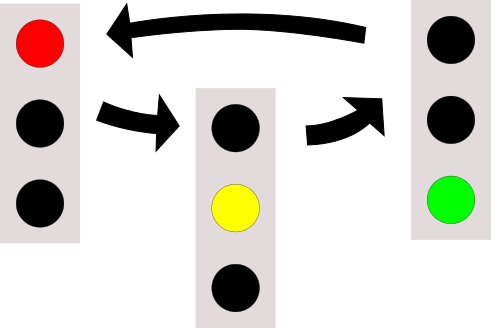
\includegraphics[width=\textwidth,keepaspectratio]
                    {./040-komponenten/010-hardware/led-default.png}
    \caption{\label{fig:led-init}}
  \end{subfigure}
  \hspace{0.1\textwidth}
  \begin{subfigure}[b]{0.40\textwidth}
    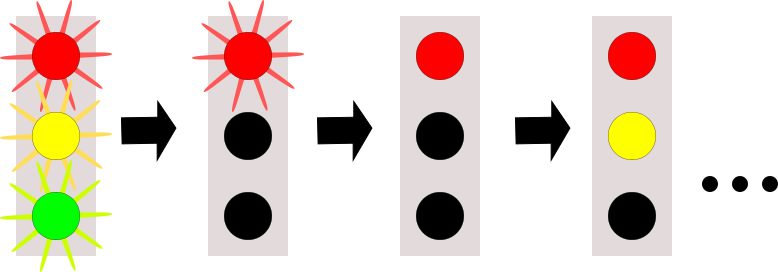
\includegraphics[width=\textwidth,keepaspectratio]{./040-komponenten/010-hardware/led-start.png}
    \caption{\label{fig:led-start}}
  \end{subfigure}
  
  \begin{subfigure}[b]{0.06\textwidth}
    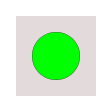
\includegraphics[width=\textwidth,keepaspectratio]{./040-komponenten/010-hardware/led-green.png}
    \caption{\label{fig:led-green}}
  \end{subfigure}
  \hspace{0.03\textwidth}
  \begin{subfigure}[b]{0.06\textwidth}
    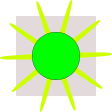
\includegraphics[width=\textwidth,keepaspectratio]
                    {./040-komponenten/010-hardware/led-green-blink.png}
    \caption{\label{fig:led-green-blink}}
  \end{subfigure}
  \hspace{0.03\textwidth}
  \begin{subfigure}[b]{0.06\textwidth}
    
\includegraphics[width=\textwidth,keepaspectratio]
                    {./040-komponenten/010-hardware/led-red-blink.png}
    \caption{\label{fig:led-red-blink}}
  \end{subfigure}
  \hspace{0.03\textwidth}
  \begin{subfigure}[b]{0.06\textwidth}
    
\includegraphics[width=\textwidth,keepaspectratio]{./040-komponenten/010-hardware/led-red.png}
    \caption{\label{fig:led-red}}
  \end{subfigure}
  \hspace{0.03\textwidth}
  \begin{subfigure}[b]{0.06\textwidth}
    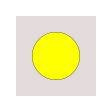
\includegraphics[width=\textwidth,keepaspectratio]
                    {./040-komponenten/010-hardware/led-yellow.png}
    \caption{\label{fig:led-yellow}}
  \end{subfigure}
  \hspace{0.03\textwidth}
  \begin{subfigure}[b]{0.06\textwidth}
    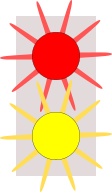
\includegraphics[width=\textwidth,keepaspectratio]
                    {./040-komponenten/010-hardware/led-red-yellow-blink.png}
    \caption{\label{fig:led-red-yellow-blink}}
  \end{subfigure}
  \caption{LED-Zustände \\ \small
           \textbf{(\subref*{fig:led-init})} Initialer Zustand
           \textbf{(\subref*{fig:led-start})} Spielstart
           \textbf{(\subref*{fig:led-green})} Spiel läuft
           \textbf{(\subref*{fig:led-green-blink})} Spielende naht \\
           \textbf{(\subref*{fig:led-red-blink})} wurde getroffen (unverwundbar)
           \textbf{(\subref*{fig:led-red})} tot
           \textbf{(\subref*{fig:led-yellow})} hat getroffen
           \textbf{(\subref*{fig:led-red-yellow-blink})} „letztes Leben“}
  \label{fig:leds}
\end{figure}
Jedes Spielgerät hat jeweils eine rote, eine gelbe und eine grüne LED, die wie auf einer Ampel
angeordnet sind.
Für Menschen mit Rot-Grün-Schwäche könnte man auch Prototypen bauen, bei denen die grüne LED durch
eine blaue LED ersetzt wird.
Mit diesen LEDs werden die verschiedenen Ereignisse kodiert.
Läuft kein Spiel und ist auch kein Spiel angekündigt, so leuchten alle LEDs der Reihe nach auf.
Dadurch können defekte, sowie nicht- oder falsch-angeschlossene LEDs schon direkt nach dem
Einschalten der Spielgeräte erkannt werden.
Wird ein Spiel angekündigt, so fangen alle LEDs an, synchron zu blinken.
10 Sekunden vor dem Spielstart blinkt dann nur noch die rote LED und 4 Sekunden davor schalten die
LEDs, analog zu einer deutschen Straßenverkehrsampel, von rot über rot-gelb auf grün.
Die grüne LED zeigt an, dass das Spiel läuft.
Dies mag zwar kompliziert klingen, ist aber doch sehr intuitiv, denn solange die grüne LED nicht
leuchtet, weiß jeder, dass das Spiel noch nicht läuft, und wenn nach rot rot-gelb kommt, weiß jeder
aus Erfahrung, dass als nächstes grün kommt.

Neigt sich das Spiel dem Ende zu, fängt die grüne LED 64 Sekunden vorher langsam an zu blinken und
blinkt bis zum Ende des Spiels immer schneller.
Dies ist natürlich nur dann der Fall, wenn der Zeitpunkt des Spielendes vorher feststeht.
Nach dem Spielende kehren die LEDs zum initialen Zustand zurück.
Wenn das Spiel läuft, zeigt das Blinken der roten LED an, dass man getroffen wurde und unverwundbar
ist.
Auch sie wird immer schneller, wenn die Zeit der Unverwundbarkeit abläuft.
Zeigt die LED Dauerrot, dann ist man tot.
In diesem Zustand ist es auch nicht mehr möglich, andere Spieler abzuschießen, d.h. der IR-Sender
wird deaktiviert.
Die gelbe LED zeigt an, dass man einen anderen Spieler getroffen hat.
Das „letzte Leben“ wird dadurch angezeigt, dass die rote und die gelbe LED etwa alle 2 Sekunden für
100 Millisekunden synchron aufleuchten.
Hierbei ist anzumerken, dass es das Konzept von „Leben“ im übertragenen Sinne nur im Spielmodus
„No Carry No Win“ in Form von Dateifragmenten gibt, wie es im \cref{sec:spielmodi-speziell}
beschrieben wird.
In Spielmodi, in denen Spieler kein „letztes Leben“ haben können, wird dieser LED-Zustand nicht
genutzt.
Alle möglichen LED-Zustände sind zur Übersicht auch in \cref{fig:leds} dargestellt.

Ursprünglich wollten wir anstelle von LEDs ganze Displays verwenden, um auch individuelle
Informationen als Text oder eine Karte des Spielfeldes mit allen Mitspielern anzeigen zu können.
Neben des begrenzten Budgets und der Tatsache, dass Informationen dieser Art auch auf der Webseite
angezeigt werden können, war auch die begrenzte Zeit ein Grund dafür, dass wir diese Idee verworfen
haben.
Auch die Karte wurde nicht umgesetzt, da für die zuverlässige und genaue Positionsermittlung eines
Spielers in geschlossenen Räumen diverse Probleme zeit- und kostenintensiv gelöst werden müssten und
dies jenseits unserer Möglichkeiten in diesem Projekt gewesen wäre.
(Trotzdem wurde zunächst viel Zeit in diese Idee investiert.)


\subsubsection{Die Hardware-API}

Dieser Abschnitt erklärt den Teil der Hardware-Komponente, die für die Kommunikation mit der
Services-Komponente sowie der Ansteuerung des Buttons und der LEDs zuständig ist.
Für diese Aufgabe war Manuel Radatz verantwortlich.

Wir haben uns dafür entschieden, dass die Hardware-Komponente und die Services-Komponente jeweils
verschiedene Programme darstellen.
Die Kommunikation erfolgt somit \textit{nicht} beispielsweise dadurch, dass von der
Services-Komponente eine Bibliothek verwendet wird, die die Hardware-Komponente bereitstellt,
sondern über Unix-Sockets.
Dabei werden Strings im Format von Google Protocol Buffers übertragen, denen jeweils ein Header mit
Nachrichten-ID und Nachrichtenlänge vorangestellt ist.
Durch die Verwendung von Protocol Buffers ist es möglich, dass die verschiedenen Komponenten in
unterschiedliche Programmiersprachen geschrieben werden können.
Dieser Flexibilität und einer besseren Wartbarkeit, die neben religiösen Gründen die Anlässe für
die Verwendung von Unix-Sockets und Google Protocol Buffers waren, stehen auf der anderen Seite ein
größerer Kommunikationsoverhead gegenüber.
Wegen der Rechenleistung der Raspberry Pis fällt dieser Overhead kaum ins Gewicht.
Da wir die gewonnene Flexibilität jedoch nicht genutzt haben und beide Komponenten in C++14
geschrieben sind, ist der Overhead letztendlich unnötig.
Rückblickend wäre es auch einfacher gewesen, wenn die Hardware-Komponente auf den Clients direkt
mit der Services-Komponente auf dem Server kommuniziert hätte, da wir uns später für eine
Client-Server-Architektur entschieden hatten.
Würde man das Projekt noch weiterentwickeln, könnte die jetzige Architektur allerdings noch von
Vorteil sein.

Die API besteht aus einem in C++14 geschriebenen Programm, welches auf allen Clients, jedoch nicht
auf dem Server läuft.
C++ war für diese Aufgabe sehr gut geeignet.
Die Sprache hat einen sehr geringen Overhead und bietet die notwendige Flexibilität.
Hauptsächlich erfolgte diese Entscheidung jedoch wegen bereits vorhandenen Programmierkenntnissen
in dieser Sprache.
Die Entscheidung für die Version C++14 beruht einfach darauf, dass dies die höchste Version ist, die
die GCC-Version, die Raspbian zur Verfügung stellt, unterstützt.
Die API kommuniziert nach oben mit dem Services-Client über Unix-Sockets und Protocol Buffers.
Nach unten kommuniziert sie mit dem Infrarot-Treiber, indem dessen Source-Code bei der Kompilierung
der API direkt eingebunden wird, und sie spricht die LEDs und den Button direkt über wiringPi an.

Für die Kommunikation nach oben wird die Socket-API der C-Standardbibliothek genutzt.
Für die Einbettung in C++ und der Nutzbarkeit nach dem in dieser Sprache üblichen RAII-Prinzip,
wurden für die Unix-Sockets und die TCP-Kommunikation der Testprogramme Wrapperklassen geschrieben,
die die Kommunikation über die Socket-API abstrahieren.
Dazu gehört auch das Puffern von unvollständigen empfangenen Nachrichten.
Alternativ hätte man auch bestehende Bibliotheken wie boost verwenden können, die ebenfalls eine
C++-Schnittstelle für die Netzwerkkommunikation zur Verfügung gestellt hätten.
Dafür hätte man sich zuerst in diese Bibliothek einarbeiten müssen und da Manuel Radatz, der diese
Komponente geschrieben hat, bereits Erfahrungen mit der C-Socket-API hatte, wäre das aufwendiger
gewesen als die Implementierung der Wrapperklassen, weshalb sie am Ende nicht genutzt wurde.
Da diese Wrapperklassen am Ende stabil liefen, war diese Entscheidung auch richtig.

Eine weitere Klasse (\texttt{InterfaceToServices}) abstrahiert die Kommunikation mit dem
Services-Client.
Sie ist hauptsächlich dafür zuständig, dass diese Kommunikation stabil bleibt und nach einem
Verbindungsabbruch (z.B. wenn der Services-Client abgestürzt ist) wieder hergestellt wird.
Bei dem Empfang von Nachrichten werden die zuvor von der \texttt{main()}-Funktion gesetzten
Callback-Funktionen aufgerufen.

Für die LED-Ansteuerung empfängt die Hardware-API vom Services-Client Nachrichten, in denen kodiert
ist, welches Ereignis wann und wie lange angezeigt werden soll.
Die Ereignisse, die übertragen werden, sind:
\begin{itemize}
  \item
    Spieler wurde getroffen und ist unverwundbar – mit der Information, wie lange der Spieler
    unverwundbar ist
  \item
    Spieler hat einen anderen Spieler getroffen – optional mit der Information, wie lange das dem
    Spieler angezeigt werden soll
  \item
    Spiel startet – mit der Information, wann das Spiel startet und wie lange das Spiel läuft
  \item
    Spiel endet – mit der Information wann
  \item
    Spieler tot
  \item
    letztes Leben
\end{itemize}
Nicht alle Ereignisse werden in allen Spielmodi genutzt.
So gibt es beispielsweise Spielmodi, in dem es das Konzept von „Leben“ nicht gibt.
Das Ereignis „Spiel endet“ ist auch nur dann notwendig, wenn bei dem Ereignis „Spiel startet“ nicht
übertragen wurde, wie lange das Spiel läuft.

Wir haben jeweils eine rote, eine gelbe und eine grüne LED, die wie auf einer Ampel angeordnet sind.
Für Menschen mit Rot-Grün-Schwäche könnte man Prototypen bauen, bei denen die grüne LED durch eine
blaue LED ersetzt wird.
Mit diesen LEDs werden die verschiedenen Ereignisse kodiert.
Läuft kein Spiel und ist auch kein Spiel angekündigt, so leuchten alle LEDs der Reihe nach auf.
Dadurch können defekte, sowie nicht- oder falsch-angeschlossene LEDs schon direkt nach dem
Einschalten der Spielgeräte erkannt werden.
Wird ein Spiel angekündigt, so fangen alle LEDs synchron an zu blinken.
10 Sekunden vor dem Spielstart blinkt dann nur noch die rote LED und 4 Sekunden davor schalten die
LEDs, analog zu einer deutschen Ampel, von rot über rot-gelb auf grün.
Die grüne LED zeigt an, dass das Spiel läuft.
Neigt sich das Spiel dem Ende zu, fängt die grüne LED 64 Sekunden vorher langsam an zu blinken und
blinkt bis zum Ende des Spiels immer schneller.
Nach dem Spielende kehren die LEDs zum initialen Zustand zurück.
Wenn das Spiel läuft, zeigt das Blinken der roten LED an, wenn man getroffen wurde und unverwundbar
ist.
Auch sie wird immer schneller, wenn die Zeit der Unverwundbarkeit abläuft.
Zeigt die LED Dauerrot, dann ist man tot.
In diesem Zustand ist es auch nicht mehr möglich, andere Spieler abzuschießen, d.h. der IR-Sender
wird deaktiviert.
Die gelbe LED zeigt an, dass man einen anderen Spieler getroffen hat.
Das letzte Leben wird dadurch angezeigt, dass die rote und die gelbe LED etwa alle 2 Sekunden für
100 Millisekunden synchron aufleuchten.

Ursprünglich wollten wir anstelle von LEDs ganze Displays verwenden, um auch individuelle
Informationen als Text oder eine Karte des Spielfeldes mit allen Mitspielern anzeigen zu können.
Neben des begrenzten Budgets und der Tatsache, dass Informationen dieser Art auch auf der Webseite
angezeigt werden können, war auch die begrenzte Zeit ein Grund dafür, dass wir diese Idee verworfen
haben.
Auch die Karte wurde nicht umgesetzt, da für die zuverlässige und genaue Positionsermittlung eines
Spielers in geschlossenen Räumen diverse Probleme zeit- und kostenintensiv gelöst werden müssten und
dies jenseits unserer Möglichkeiten in diesem Projekt gewesen wäre.
(Trotzdem wurde zunächst sehr viel Zeit in diese Idee investiert.)

Die LED-Ansteuerung erfolgt ebenfalls in einer eigenen Klasse namens \texttt{LEDEventStatus}.
Diese ruft direkt Funktionen von wiringPi auf, verwaltet alle Daten, die zur korrekten
LED-Ansteuerung notwendig sind (auch die Timer) und interpretiert als Eingabe das von Services
empfangene Zahlentripel.

Der Status des Button wird direkt in der \texttt{main()}-Funktion durch Aufrufe der
wiringPi-Funktionen abgefragt.

Die \texttt{main()}-Funktion besteht abgesehen von der Initialisierung aus einer Schleife, die erst
dann beendet wird, wenn das Programm \texttt{SIGTERM} empfängt.
Dort besteht jede Iteration aus:
\begin{itemize}
  \item
    das Abfragen, ob Nachrichten vom Services-Client angekommen sind, welche dann auch durch das
    Aufrufen von Callback-Funktionen interpretiert werden,
  \item
    die Aktualisierung des LED-Status,
  \item
    die Abfrage des Buttons, ob dieser gedrückt wird, wobei in diesem Fall die eigene Client-ID an
    den IR-Sender gesendet wird und
  \item
    das Abfragen des IR-Sensors, ob Daten empfangen wurden sowie die Weiterleitung dieser an den
    Services-Client.
\end{itemize}
Danach wartet das Programm 0,5 Millisekunden, um die CPU-Auslastung gering und folglich die
Temperatur des Prozessors niedrig zu halten und die Lebensdauer des Akkumulators zu erhöhen.
Die dadurch entstehende Latenz von bis zu 0,5 Millisekunden ist so niedrig, dass sie keine spürbaren
Auswirkungen auf das Spiel haben sollte.
Wird der Button gedrückt, werden auch nicht in jeder Iteration IR-Daten gesendet.
Dies würde zu einer Überbeanspruchung der IR-LED führen.
Stattdessen werden ab dem Moment, in dem der Button heruntergedrückt wird, nur alle 100
Millisekunden IR-Daten an den IR-Treiber übergeben.

Neben diesem regulären Ablauf wurden auch zahlreiche Features zum Testen implementiert, welche über
Programmparameter ein- oder ausgeschaltet werden können.
Ist kein Button vorhanden, so besteht die Möglichkeit, dass ohne Unterbrechung alle 500
Millisekunden die eigene Client-ID an den IR-Sender gesendet wird.
Wenn kein IR-Empfänger funktionsfähig ist, das Programm auf anderer Hardware ausgeführt wird oder
nur die Kommunikation mit dem Services-Client getestet werden soll, gibt es zusätzlich einen
automatischen und einen manuellen Testmodus.
Im automatischen Testmodus werden regelmäßig zufällige Daten an den Services-Client gesendet, als
wären diese von dem IR-Sensor empfangen worden.
Im manuellen Testmodus kann man manuell Testdaten eingeben, die gesendet werden sollen.
In beiden Testmodi wird der LED-Status auch auf der Konsole ausgegeben.
Dadurch sind Tests auch ziemlich einfach in virtuellen Umgebungen ohne die Hardware möglich.

Außerdem wurden Stubs implementiert, welche den Services-Client ersetzen können, sodass auch
andersherum die Hardware ohne Services getestet oder demonstriert werden kann.
Dazu gehört ein Stub, der LED-Ereignisse an die Hardware-API sendet und ein Paar von Stubs, von
denen einer auf den Clients und einer auf dem Server läuft, der alle empfangenden IR-Daten auf dem
Server ausgibt.

Die Hardware-API läuft im fertigen System als Daemon.
Sie kann aber auch als gewöhnliches Programm gestartet werden, was zum Testen auch notwendig ist.

Der build-Prozess erfolgt durch eine einzige Makefile.
Wegen der Einfachheit des Programms und der Tatsache, dass die Programme gezielt für ein bestimmtes
System entwickelt worden sind, wäre die Nutzung von cmake oder des GNU Build Systems überflüssig
gewesen.



\subsection{Services}
\label{sec:services}

Mitglieder und Aufgaben:
\begin{itemize}
  \item
    Angelina Jellinek (Design der Webseite und Website Backend)
  \item
    Jan Arne Sparka (Integration von LUA und Server)
  \item
    Kevin Marc Trogant (Integration von Hardware und Server)
  \item
    Pascal Jochmann (Website Backend, Client-Server Kommunikation)
  \item
    Tim Sikatzki (Website Backend und Datenbank)
\end{itemize}

\subsubsection{Aufbau}
Das gesamte Netzwerk ist über eine zentrales System realisiert. Die einzelnen 
Clients kommunizieren nicht untereinander, sondern alle mit dem Server, der die Spielverwaltung übernimmt. 
Die Einstellungen der Spielparameter und die Darstellung des Punktestandes übernimmt eine Website, die auf dem Server läuft. 
Auf dieser können die Spieler Dinge wie Spieleranzahl und Rundendauer festlegen; außerdem meldet 
die Website dem Server den Start des Spiels. Zuletzt gibt es noch eine Datenbank zur Festhaltung des Punktestandes. 
Sie wird vom Server aktuell gehalten und von der Website auf einem Scoreboard dargestellt.

\subsubsection{Kommunikation}
Dieser Abschnitt erläutert, wie die Hardware mit dem Server kommuniziert, sowie den Aufbau der Software beider Geräte.
Für diese Aufgabe war Kevin Marc Trogant verantwortlich. Für Teile der Kommunikation zwischen Server und Client außerdem Pascal Jochmann.

Der Spielserver \texttt{services-server} nutzt einen eigenen Thread für die Kommunikation mit den Clients und
der Webseite. Clients und Server kommunizieren über BSD Sockets.
Als Alternative kam Googles gRPC in Frage. Dieses wurde verworfen, weil:
\begin{itemize}
    \item gRPC erlaubt Kommunikation nur in eine Richtung. Der Server kann nur dann Nachrichten an den Client verschicken,  wenn ein Request eingegangen ist.
    \item gRPC erlaubt nur einen Nachrichtentypen pro Kommunikationsrichtung. Da wir mehrere verschiedene Nachrichtentypen benötigen, hätten wir das Konzept eines Unions in gRPC nachbilden müssen.
\end{itemize}
Es wäre möglich gewesen, Bibliotheken, zum Beispiel \href{http://think-async.com/Asio/WebHome}{boost.asio}, die eine einfachere Schnittstelle anbieten, zu verwenden. Da wir zu dem Zeitpunkt, an dem wir entschieden haben, die Socket API direkt zu verwenden, noch nicht genau wussten, wie die Netzwerkkommunikation funktionieren würde, wollten wir uns möglichst viele Optionen offen halten. Außerdem hatten wir im Verlauf der Entwicklung mehrmals Probleme mit inkompatiblen Bibliotheksversionen, entweder durch andere APIs oder – wesentlich lästiger – durch unterschiedliches Verhalten. Deshalb waren wir später sehr zurückhaltend beim Einführen neuer Abhängigkeiten.

An die Datenbank ist der Server über die \href{https://dev.mysql.com/doc/connector-c/en/connector-c-introduction.html}{mysql c connector} Schnittstelle angebunden. Die Schnittstelle bietet eine relativ simple API: Zuerst verbindet sich das Programm mit dem MySQL Datenbankserver (entweder über TCP oder über Unix Sockets) und dann können beliebige SQL Anfragen als String an den Datenbankserver geschickt werden, der daraufhin Zeilenweise die Ergebnisse zurückliefert.
Diese Schnittstelle ist in einem C++ Singleton gekapselt \texttt{DatabaseConnection}, die Methoden für alle Anfragen
bereitstellt, die der Server stellen muss (bswp \texttt{get\_runnable\_games()}). \newline
\newline
Der Thread für die Kommunikation führt in einer Endlosschleife folgende Schritte aus:
\begin{enumerate}
    \item Falls sich neue Clients verbunden haben: Lege die passenden Datenstrukturen an und setze den Status des Clients in der Datenbank auf verbunden.
    \item Hole eine Liste noch nicht beendeter Spiele von der Datenbank. Falls neue dazu gekommen sind, lege ein entsprechendes Objekt an.
    \item Frage den aktuellen Zustand aller Spiele, die dem Server bekannt sind, ab. Falls ein Spiel gestartet wurde, starte den entsprechenden Thread für die LUA API des Spiels.
    \item Sende den Spiellogik-Threads aller neu beendeten Spiele eine Nachricht, die diese dazu auffordern, sich zu beenden.
    \item Empfange und parse Nachrichten von Clients. (Siehe weiter unten)
    \item Zurück zu 1.
\end{enumerate}

Damit Spielereignisse an den Spieler kommuniziert werden können, kann die Spiellogik Funktionen auf dem Server aufrufen, die dafür sorgen, dass passende Nachrichten an die Clients gesendet werden. Dazu gibt es einen Nachrichtentyp, in dem mittels eines Enums kodierte LED-Befehle enthalten sind. 

Das Nachrichtenformat ist mittels Google Protocol Buffers, Googles Lösung der Datenformatserialisierung umgesetzt. Dies ist eine sehr simple Lösung der Frage, wie wir die Nachrichten einheitlich und verständlich strukturieren. Protocol Buffers ist dabei im Vergleich zu den betrachteten Alternativen wie XML am simpelsten mit dem wenigsten Overhead, während es trotzdem unseren Anforderungen genügt.\\
 Da Protocol Buffers jedoch selbst keine Möglichkeit
implementiert, um aus einem empfangenem Byte-String den Nachrichtentyp zu rekonstruieren, wird vor jeder Nachricht
ein Header verschickt, der den Nachrichtentyp und die Länge der Nachricht in Bytes enthält.
Die Nachrichten selbst können einfach mittels der Protocol-Buffers Bibliothek zu entsprechenden C++ Objekte geparst werden, die dann Nachrichtenfelder als \glqq Getter- und Setter-Funktionen\grqq \, verfügbar machen.

Die Kommunikation mit der Hardware-Komponente läuft über eine eigene Komponente (\texttt{services-client}), die auf den Spielgeräten ausgeführt wird. Diese empfängt Nachrichten von der Hardware-Schnittstelle über einen Unix-Socket, wandelt diese in das Services-interne Format um und sendet sie dann über einen TCP Socket an den Server. Außerdem kümmert sich die Komponente darum, in regelmäßigen Abständen (ca. 5 Sekunden) eine kurze \glqq Keep-Alive\grqq \, Nachricht an den Server zu senden, um zu signalisieren, dass der Client noch verbunden ist und am Spielbetrieb teilnimmt. 
Eingehende Nachrichten vom Server, zum Beispiel um mittels der auf dem Gerät vorhandenden LEDs Treffer etc. anzuzeigen, werden vom Client empfangen und an die Hardware API weitergeleitet.\newline \newline
Da für ein Lasertag das Treffen von anderen Spielern von relativ hoher Bedeutung ist, soll hier noch kurz ausgeführt werden, was aus Sicht der Services-Komponente passiert, wenn ein Spieler einen anderen trifft.

Zuerst erhält der Client eine Nachricht von der Hardware-API, die mitteilt, dass der Client getroffen wurde. In der Nachricht ist die ID des Clients enthalten, von der das Gerät getroffen wurde. Die eigene ID erhält der Client beim Start. Diese beiden Informationen werden in eine sog. \glqq Hit-Message\grqq \, verpackt und an den Server gesendet. 
Der Server erhält die Nachricht, parst diese und sucht nach einem Spiel, das beide Clients – Schießenden und Getroffenen – enthält. Findet er kein passendes Spiel, wird die Nachricht verworfen. Falls ein passendes Spiel gefunden wurde, werden die Client-IDs zu den entsprechenden Spieler-IDs aufgelöst (die Zuordnung ist pro Spiel eindeutig) und eine passende Nachricht an den entsprechenden Spiel-Thread geschickt.

\subsubsection{LUA API (services)}
Dieser Abschnitt erläutert, wie die LUA API mit dem Server kommuniziert. Für diese Aufgabe war Jan Arne Sparka verantwortlich.

Um Spielmodi zu beschreiben und sauber von den anderen Komponenten abzutrennen brauchten wir eine API. Die erste Entscheidung war zwischen LUA, c-Code und einer eigenen Spielmodus-DSL. Da unsere Spiellogikgruppe die Entscheidung für LUA traf und sogar schon einen funktionierenden Simulator für Spiele in sehr schneller sukzession herausbrachte, war diese Entscheidung für uns damit schnell getroffen.

Die LUA API auf services Seite war sehr schwierig einzubauen. Die erste Option war es die API als Singleton bereitzustellen, dies stellte sich aber sehr schnell als schlechter Ansatz heraus, da der Start einer weiteren Runde hierdurch zu einem komplizierten und unschönen Hack geworden wäre. Daher und da wir die Architektur für potentiel mehrere Spiele die Parallel laufen offen halten wollten, entschieden wir uns für den jetztigen Ansatz, die API läuft in einem eigenen Thread. 

Der Logik-Thread sammelt sich erstmal die relevanten Spieldaten zusammen, initialisiert dann die Felder auf welche LUA zugreift und geht dann in eine Event Loop über. In dieser Gameloop wird zuerst überprüft ob Schussnachrichten durchgereicht wurden, welche wiederum an LUA weitergereicht werden. Danach werden alle potentiellen Timer weitergetickt um die vergangene Zeit. Als letzte wird noch abgeprüft ob der Server uns ein AskedToExit Event schickt, welches mit Aufräumen und beenden des Spiels quittiert wird.

Der Hauptteil der API Arbeit auf der service Seite war die vorhandene Spiellogik API (den Simulator) an die real genutzte Hardware und Software anzubinden. Der Großteil der Input/Output Operationen wurde über unser Datenbankconnection Singleton umgeleitet. Das Scoreboard wird dabei permanent mitgeführt, wodurch Erweiterungen, wie z.B. spielerseitige Displays denkbar sind und was uns die Probleme von Score Serialisierung ignorieren lässt, da dieser sowieso von der Datenbank serialisiert wird. Da dann letztendlich die Relevanz eines Timers für LUA Skripte aufkam, welcher nicht den Logik-Thread vom Arbeiten abhält, haben wir einen einfachen Timer entwickelt der mit Funktionen Callbacks arbeitet. Die letzte Erweiterung der API war das hinzufügen der LED Events und der Abstraktion dieser in Funktionen, die Teil der LUA API wurden.

Die services Seite der LUA API hatte als Hauptproblem, das sie aufgrund der sehr zentralen Stellung (Verknüpfung von 3 Komponenten), sehr viele Abhängigkeiten hatte und sehr schwierig zu testen war. Dies ist dem Projekt letztendlich zum Verhängnis geworden, da wir in der Interaktion dieser vier Komponenten einen Fehler haben, den wir bisher noch nicht lokalisieren konnten. Das Debugging ist auf Grund von LUA auch nur sehr begrenzt möglich und wird uns noch einiges an Aufwand einbringen.
\shorthandoff{"}
\subsubsection{Website}
Dieser Abschnitt erläutert, wie die Website aufgebaut ist und funktioniert. Für diese Aufgabe waren Tim Sikatzki, Angelina Jellinek und Pascal Jochmann verantwortlich.

Unsere Website bildet das Herzstück in der Interaktion zwischen dem Nutzer und der Software. Sie gibt ihm die Möglichkeit, die Konfigurationen für das Spiel einzustellen, wie zum Beispiel die Anzahl der Teams, dem Spielmodus und den Spielgeräten Namen zuzuteilen. Außerdem haben die Spieler durch sie die Möglichkeit, ihre Leistungen während des Spiels in Echtzeit einsehen zu können.\\\\
Zur Entwicklung der Website haben wir "Flask" benutzt, ein Webframework auf Python-Basis. Wir haben uns für dieses Framework entschieden, da es zunächst sehr leicht zu benutzen ist und uns gleichzeitig alles geboten hat, um die erwarteten Funktionalitäten der Website implementieren zu können, wie zum Beispiel ein MySQL-Package, welches wir zur Interaktion zwischen Webapplikation und Datenbank benutzt haben.
Um die oben genannten Funktionen gewährleisten zu können, besteht unsere Webapplikation aus mehreren HTML-Seiten.\\\\
Die erste Seite (\cref{fig:start}) ist der Kern der Website. Sie wird benutzt, um das eigentliche Spiel zu erstellen. Nicht nur nimmt sie die eingegebenen Daten der Spieler auf, sondern überträgt die Einstellungen direkt auf die Datenbank und erstellt dort direkt Einträge, die für das Scoreboard relevant sind. In der Sektion Datenbank werden die Einträge und Tabellen genauer erläutert. Die möglichen Einträge der Spielernamen sind hierbei abhängig von der Anzahl der verbundenen Clients. Sind nur drei Clients zum Server verbunden, so können wir auch nur drei Namen zuweisen.
Auch die Spielmodi, die ausgewählt werden können, werden dynamisch erstellt. Hierbei wird aus einem Ordner ausgelesen, in dem die Lua-Skripte abgelegt werden können. Die Teams werden von der Webapplikation mithilfe von einer Modulo-Operation, abhängig von der Teamanzahl, automatisch zugeteilt. Es ist also \\\\
Sobald ein Spiel gestartet wird, leitet die Seite auf das Scoreboard weiter.\\ Das Scoreboard zieht sich seine Einträge direkt aus der Datenbank und aktualisiert dieses asynchron unter der Verwendung von JavaSyript (unter Verwendung von jQuery) und ajax. Es stellt die Einträge in Form von Tabellen da, hierbei gibt es eine Tabelle die Spieler und eine Tabelle für die Teams (\cref{fig:team}). Auf der Seite haben wir dann die Möglichkeit, das Spiel manuell zu pausieren oder auch zu beenden. Wenn die Dauer einer Runde ausgelaufen ist, wird das Spiel automatisch in den pausierten Zustand gesetzt. Wir können nun jederzeit eine mithilfe des Links "Spiel fortfuehren" Eine neue Runde starten bzw. das pausierte Spiel weiterspielen.\\
Der Link "Spiel beenden" funktioniert dementsprechend genauso, allerdings ist es danach nicht mehr möglich, das Spiel weiterzuführen. Der Nutzer dann danach auf einen Button klicken, um zurück zur Startseite zu gelangen und ein neues Spiel zu starten .\\\\
Insgesamt ist die Webapplikation seitens Funktionalität vollständig. Es könnten noch Verbesserungen hinsichtlich der Anzeige der verschiedenen Dateifragmente und der Effizienz der Anzeige des Scoreboards gemacht werden.


\subsubsection{Style}

\begin{figure}[htb]
	\begin{center}
		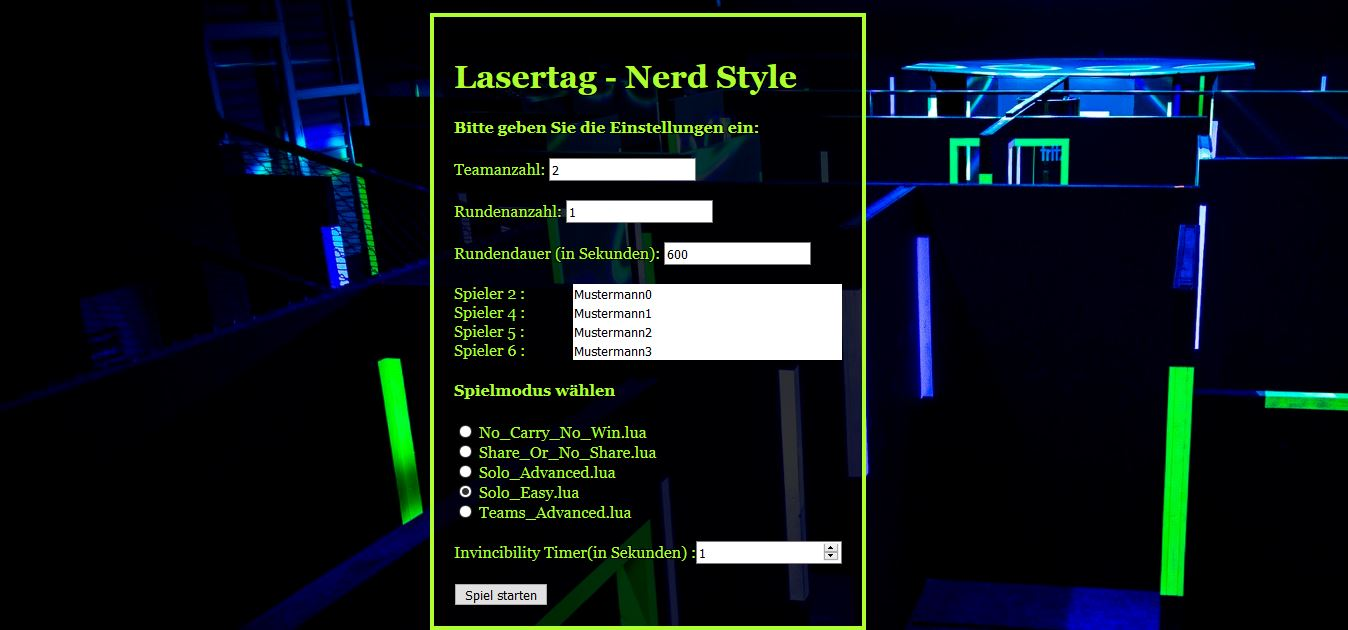
\includegraphics[width=0.75 \textwidth]{websitemenue.JPG}
		\caption{Startseite}
		\label{fig:start}
	\end{center}
\begin{center}
	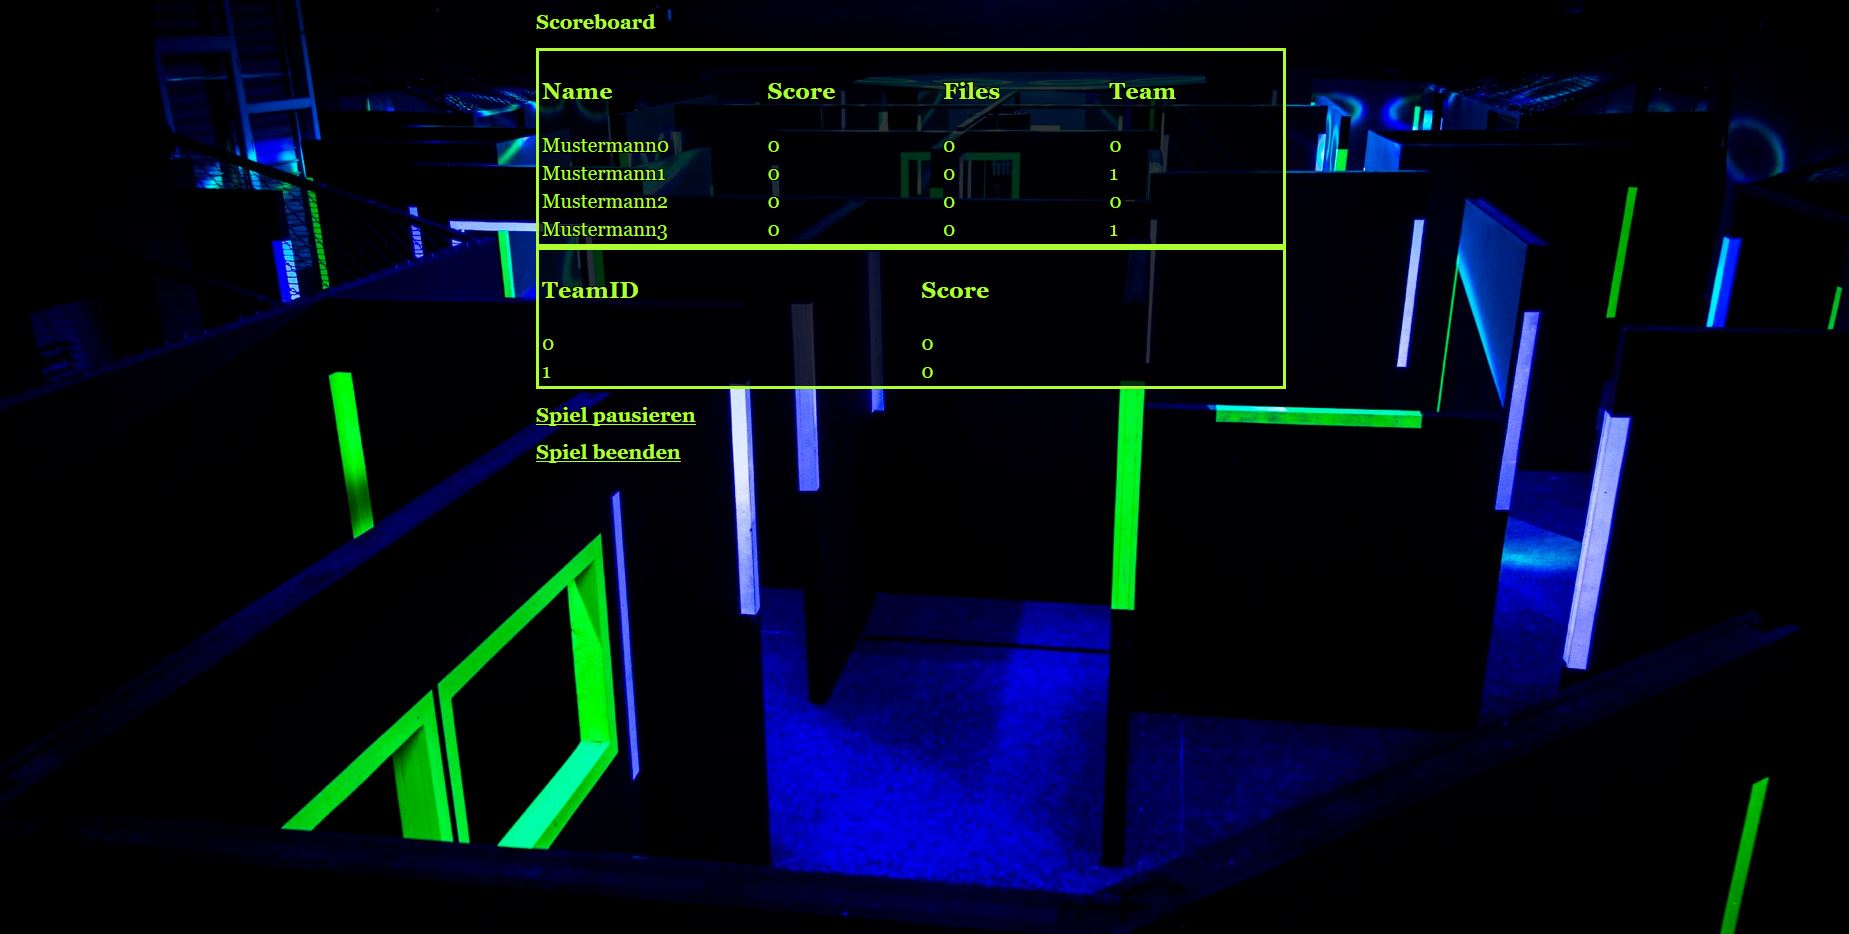
\includegraphics[width=0.75 \textwidth]{scoreboardteams.JPG}
	\caption{Scoreboard mit Teams}
	\label{fig:team}
\end{center}
\end{figure}
%\begin{figure}[b]
	
%\end{figure}
Dieser Abschnitt erläutert, wie die Website gestaltet wurde. Für diese Aufgabe war Angelina Jellinek verantwortlich.

Viele Styleformatierungen sind auf der Scoreboardseite genau wie auf der Startseite. Es gibt jedoch auch noch einige Besonderheiten. Da sich das Scoreboard regelmäßig aktualisiert mussten wir die Links zu der gestoppten und pausierten Seite so designen, dass er im „Originalzustand“ und „angeklicktem Zustand“ genau gleich aussieht und nicht als Link erkennbar ist.
Das Aussehen der Website ist  dynamisch gestaltet. Die Größe des Scoreboards passt sich individuell an die Anzahl der Einträge an. Auch die Box passt sich dynamisch an die Einträge an. Gleichzeitig gibt es auch nur ein extra Scoreboard für Teams, wenn es Teams auch wirklich gibt.\\ Sowohl der Hintergrund, als auch die Schriftart und die Farben sind so gewählt, dass sie zum Thema Lasertag und Nerd Style passen. 
Die Schrift ist in grün gehalten, damit ein guter Kontrast zwischen Hintergrund und Text entsteht. Der Hintergrund dieser Textfelder hat eine leicht schwarze Transparenz bekommen, damit die grüne Schrift auch auf helleren Stellen des Hintergrunds der Website gut lesbar ist. Alle Textfragmente einer Seite befinden sich in einer Box, um die Position auf der Seite bestimmen zu können, ohne kleine Unregelmäßigkeiten der Einrückungen zu bekommen. Es stehen mehrere Schriftarten zur Auswahl, von denen die erste angewendet wird, die dargestellt werden kann. Hier handelt es sich um die Schriftarten Georgia und Times New Roman. Das Design dunkel genug und wenig belastend für die Augen, um es in einer dunklen Halle auf eine Leinwand zu übertragen, ohne dabei die Spieler von ihrem Spiel abzulenken. \\\\


\subsubsection{Datenbank}
\begin{figure}[htb]
	\begin{center}
		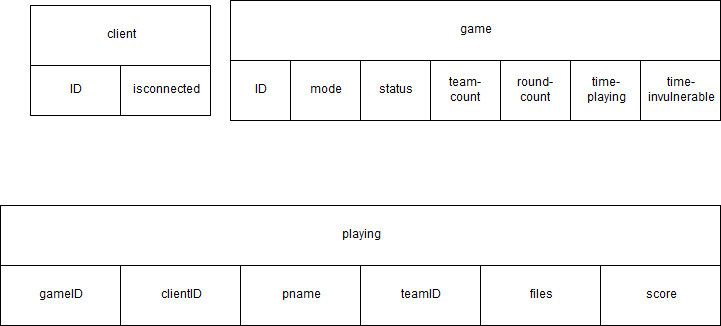
\includegraphics[width=0.8 \textwidth]{Databasestrucb.png}
		\caption{Datenbankstruktur}
		\label{fig:database}
	\end{center}
\end{figure}
Dieser Abschnitt erläutert, wie die Website mit der Datenbank zusammenarbeitet. Für diese Aufgabe war Tim Sikatzki verantwortlich.

Unsere Datenbank ist die ermöglichte uns die Interaktion innerhalb der services-Gruppe. Wir haben uns für eine Datenbank entschieden, da wir eine Spielhistorie aus den vergangenen Spielen erstellen wollten. Gleichzeitig bot sich die Datenbank auch für die Darstellung des Scoreboard an, da die SQL Anfragen für eben dieses sehr trivial waren.\\\\
Um die Fehlerquelle einer Datenbank in Form einer Datei zu umgehen, haben wir uns nach einiger Zeit dafür entschieden von SQLite auf MySQL, als Datenbankmanagementsystem, umzusteigen.\\\\
%Abbildung mit Tabellen hier einfügen

In der Grafik (\cref{fig:database}) sehen wir den Aufbau unserer Datenbank. Wie wir sehen können, ist sie in drei Tabellen unterteilt.\\
Die client - Tabelle ist relevant für das Anzeigen der möglichen Eingabefelder für die Spielernamen im Menü der Website. Hierbei wird unterschieden, ob ein Client mit dem Server verbunden ist oder nicht.\\\\
Die game - Tabelle ist vorallem interessant für die LUA API, da sie die Einträge enthält, die von dem Spieler vor Beginn des Spieles mithilfe des Menüs übergeben werden, wie zum Beispiel der Spielmodus und die Rundendauer. Gleichzeitig beinhaltet die Tabelle auch den Status, den das jeweilige Spiel zu jeder Zeit hat. Dieser Status wird von allen Parteien benutzt: die LUA API muss das Spiel nach Überschreiten der Rundendauer pausieren oder es beenden, die Netzwerkkommunikation muss bei einem gestoppten Spiel aufhören, Nachrichten weiterzuschicken, damit keine Punkte während eines pausierten oder beendeten Spieles verteilt werden.\\\\\\
Die "playing" - Tabelle wird für unsere Historie und gleichzeitig der Darstellung des Scoreboards benutzt. Sie teilt jedem Spieler eine gameID, den jeweiligen Score, die Dateifragmente usw. zu und macht es möglich die Tabelle nach der gameID zu sortieren um einzelne Spiele wieder einsehen zu können.

\shorthandon{"}
\subsubsection{Debugging}

Um Fehler zu finden und das Verhalten des Systems nachvollziehen zu können, geben sowohl Client als auch Server Log-Ausgaben auf \texttt{stderr} aus. Da beide von systemd gestartet werden, können diese Log-Ausgaben auch mit den üblichen Systemd-Kommandos angezeigt werden.\newline

Zusätzlich zu den genannten Arbeitsaufteilungen fanden regelmäßige Gruppentreffen aller Mitglieder statt bei denen es primär um Abstimmung der Arbeit ging. Auf diesen Treffen wurden jedoch auch gemeinsam der allgemeine Aufbau unserer Komponenten, das Datenbankmodell und ähnliches (weiter)entwickelt, außerdem gemeinsames Bugfixing.



\subsection{Spiellogik}
\label{spiellogik}

Mitglieder und Aufgaben:
\begin{itemize}
  \item
    David Bachorska (Entwicklung eines Spielmodus, Erweiterung des Simulators)
  \item
    Dennis Ness (Entwicklung eines Spielmodus, grundlegende Implementierung des Simulators)
  \item
    Tom Kieseling (Entwicklung eines Spielmodus, Erweiterung des Simulators)
\end{itemize}


\subsubsection{Spielmodi allgemein}
Die wichtigste Anforderung seitens des Kunden für die Umsetzung der Spielmodi war, dass eines oder mehrere Ad-Hoc Multi-Hop Netzwerkprotokolle diesen zugrundeliegen sollten. Dabei sollen die Entscheidungen für Interaktionen von den Spielenden möglichst selbst getroffen werden, damit die Spielenden lernen können, wie das jeweils gespielte Netzwerkprotokoll funktioniert. Darüberhinaus war dem Kunden jedoch auch die Spielbarkeit (Fairness, Spannung, Unterhaltung) wichtig. Als Vorbild in diesem Zusammenhang sollte Lasertag dienen. Es war dem Kunden und auch uns dabei klar, dass das Modifikationen am jeweiligen Netzwerkprotokoll erforderlich machen würde.

Als Ideen für die Umsetzung dieser Anforderungen standen zwei grobe Szenarien zur Diskussion: ein Protokoll aus dem Bereich der Wireless Sensor Networks oder der Peer-to-Peer Content Distribution. Nach eingehender Beschäftigung mit einigen Protokollen aus dem Bereich der Wireless Sensor Networks gab es erhebliche Zweifel an der Umsetzbarkeit eines Spiels auf deren Basis unter Berücksichtigung der genannten Spielbarkeitskriterien Spannung und Unterhaltung und nach dem Vorbild von Lasertag. So besteht ein Wireless Sensor Network meist aus vielen Wireless Sensor Nodes, die gut von den Spielenden repräsentiert hätten werden können. Jedoch arbeiten diese Knoten in der Praxis oft zusammen an der Erfüllung eines gemeinsamen Ziels. Wir haben keinen Konkurrenzgedanken, keine egoistischen Motive der einzelnen Netzwerkknoten in Wireless Sensor Networks gesehen, die sich gut zur Umsetzung eines Spiels nach dem Vorbild von Lasertag geeignet hätten. Stattdessen gibt es Ziele in Wireless Sensor Networks wie die Energiesparsamkeit der einzelnen Geräte, deren Umsetzung für uns im Widerspruch zu einem action-geladenen Spiel wie Lasertag standen. Das Spiel auf dieser Basis wäre eher statisch geworden.

Nach Beschäftigung mit Peer-to-Peer Content Distribution erschien diese uns deutlich besser als Grundlage für das Spiel geeignet. Wir haben uns dabei für den bekanntesten Vertreter seiner Art, BitTorrent, entschieden, denn wir haben folgende Analogien zwischen dessen Funktionsweise und Lasertag gefunden, die sich durch alle von uns erstellten Spielmodi ziehen:

\begin{enumerate}
\item Bei Lasertag interagieren die Spielenden miteinander, indem sie mit ihrer Spielwaffe auf die Weste eines anderen Spielenden schießen. Diese Interaktion, der Schuss, entspricht in unserem Spiel im Sinne von BitTorrent der Initiierung einer Datenübertragung zwischen den beiden Spielenden. Der Schuss zwingt den Getroffenen im Allgemeinen zur Übertragung eines Dateifragments an den Schützen. Dabei wird der Einfachheit halber automatisch das erste Dateifragment ausgewählt, das der Schütze noch nicht hat. Sollte es kein solches Dateifragment geben, dass der Getroffene besitzt und der Schütze noch nicht, so ändert sich entsprechend nichts an den Dateifragmenten beider Spieler.

Anmerkung: Da es sich um ein Spiel handelt, wird nicht wirklich ein Dateifragment übertragen, sondern lediglich die Information über dessen (theoretischen) Besitz.

\item Bei Lasertag hat jeder Spielende standardmäßig das (egoistische) Ziel, möglichst viele seiner Gegner zu treffen bzw. abzuschießen, und er bekommt dafür Punkte. Bei BitTorrent hat jeder Teilnehmer im Netzwerk das (ebenfalls egoistische) Ziel, möglichst schnell die gewünschte Datei(en) von seinen Peers vollständig zu erhalten. Entsprechend vergeben wir im Allgemeinen (wenn nicht anders beim jeweiligen Spielmodus erklärt) auch in unserem Spiel Punkte für erfolgreiche und für das Erreichen des egoistischen Ziels sinnvolle Interaktionen, also Datenübertragungen zwischen den Peers.

\item Bei Lasertag gibt es das Konzept der Unverwundbarkeitszeit. Wenn ein Spielender einen anderen Spielenden getroffen hat, dann ist der Getroffene üblicherweise für eine gewisse Zeit (einige Sekunden) vor weiteren Schüssen auf ihn geschützt. Das verhindert unfairen Mehrfachbeschuss von einem Spieler innerhalb kurzer Zeit. Diese Zeit kann der Getroffene nutzen, um sich selbst wieder in Deckung zu begeben.

Wir haben dieses Konzept im Prinzip aus denselben Gründen in unsere Spielmodi übernommen. Im Kontext von BitTorrent lässt sich diese Unverwundbarkeitszeit jedoch auch einfach als die Zeit erklären, die die durch den Schuss initiierte Datenübertragung (für ein Dateifragment) benötigen würde. In unserem Spiel kann dieser Interpretation folgend jeder Schütze zwar mehrere Dateifragmente gleichzeitig erhalten, jedoch kein Getroffener mehr als ein Dateifragment gleichzeitig an einen oder mehrere Schützen übertragen. Natürlich wären in der Realität bei BitTorrent mehrere Datenübertragungen in beide Richtungen gleichzeitig möglich und sogar anzustreben. Die genannte Interpretion ist also gleichzeitig eine der Vereinfachungen, die wir zur besseren Spielbarkeit vorgenommen haben.

\item Bei Lasertag gibt es Spielmodi in Teams. Dieses Spiel in Teams lässt sich gut zur Darstellung des kollaborativen Ansatzes von BitTorrent nutzen. Denn trotz der egoistischen Motive der Peers im Netzwerk braucht jeder Peer die anderen Peers und trägt entsprechend auch selbst etwas zur Erreichung der Ziele anderer Peers bei, indem er ihnen bereits erhaltene Dateifragmente zur Verfügung stellt.
\end{enumerate}

\noindent
Allgemein folgen all unsere Spielmodi den folgenden Annahmen. Diese sind größtenteils Vereinfachungen, die die Komplexität des Spiels reduzieren und es damit leichter spielbar machen.

\begin{enumerate}
\item Jeder Spielende besitzt zum Start ein Dateifragment, welches keiner seiner “Peers” (alle anderen Spielenden) besitzt.
\item Es geht insgesamt um eine Datei, die in entsprechend viele Dateifragmente zerlegt ist, wie es Spielende im Spiel gibt.
\item Ziel ist allgemein, bis auf Ausnahmen, die beim entsprechenden Spielmodus beschrieben sind, die eine Datei als Erster vollständig von den Peers zu erhalten.
\end{enumerate}

\noindent
Die initiale Verteilung der Dateifragmente auf die Peers sorgt für einen schnellen und relativ einfachen Einstieg in das jeweilige Spiel, weil sich so zu Beginn ein Schuss auf jeden Peer lohnt. Entsprechend nimmt die Komplexität des Spiels für jeden Spielenden mit der Zeit zu. So muss jeder Spielende zunehmend im Auge behalten, welche Dateifragmente er schon hat und von welchem Peer er die fehlenden bekommen kann.

Wir haben verschiedene Spielmodi entworfen, die grundsätzlich auf den genannten Analogien und Annahmen beruhen. Sie unterscheiden sich teilweise in der Komplexität ihrer Regeln und haben teilweise verschiedene Szenarien als Ausgangspunkt, die entsprechenden Einfluss auf das Spiel und dessen Regeln nehmen.
\subsubsection{Spielmodi speziell}
\label{sec:spielmodi-speziell}

Die verschiedenen Spielmodi wurden mittels eines von uns als Simulator bezeichneten Programms entwickelt und ausprobiert. So konnten wir u.a. prüfen, ob die Spielmodi wie erwartet funktionieren und ob bei realistischen Eingaben (also entsprechenden Schusswechseln zwischen den Spielern) Szenarien auftreten können, die entsprechend der Bedeutung des jeweiligen Spielmodus nicht sinnvoll sind. \\
Der Simulator ist kommandozeilenbasiert. Er ermöglicht alle wichtigen Eingaben, die im fertigen Produkt über die Webseite möglich sein sollten, u.a. der gewünschte Spielmodus, die Anzahl der Spieler, die Anzahl der zu spielenden Runden und die Unverwundbarkeitszeit. Lediglich Spielernamen kennt der Simulator nicht. Die simulierten Spieler werden einfach von 0 beginnend durchnummeriert.
\begin{figure}[h]
  \centering
  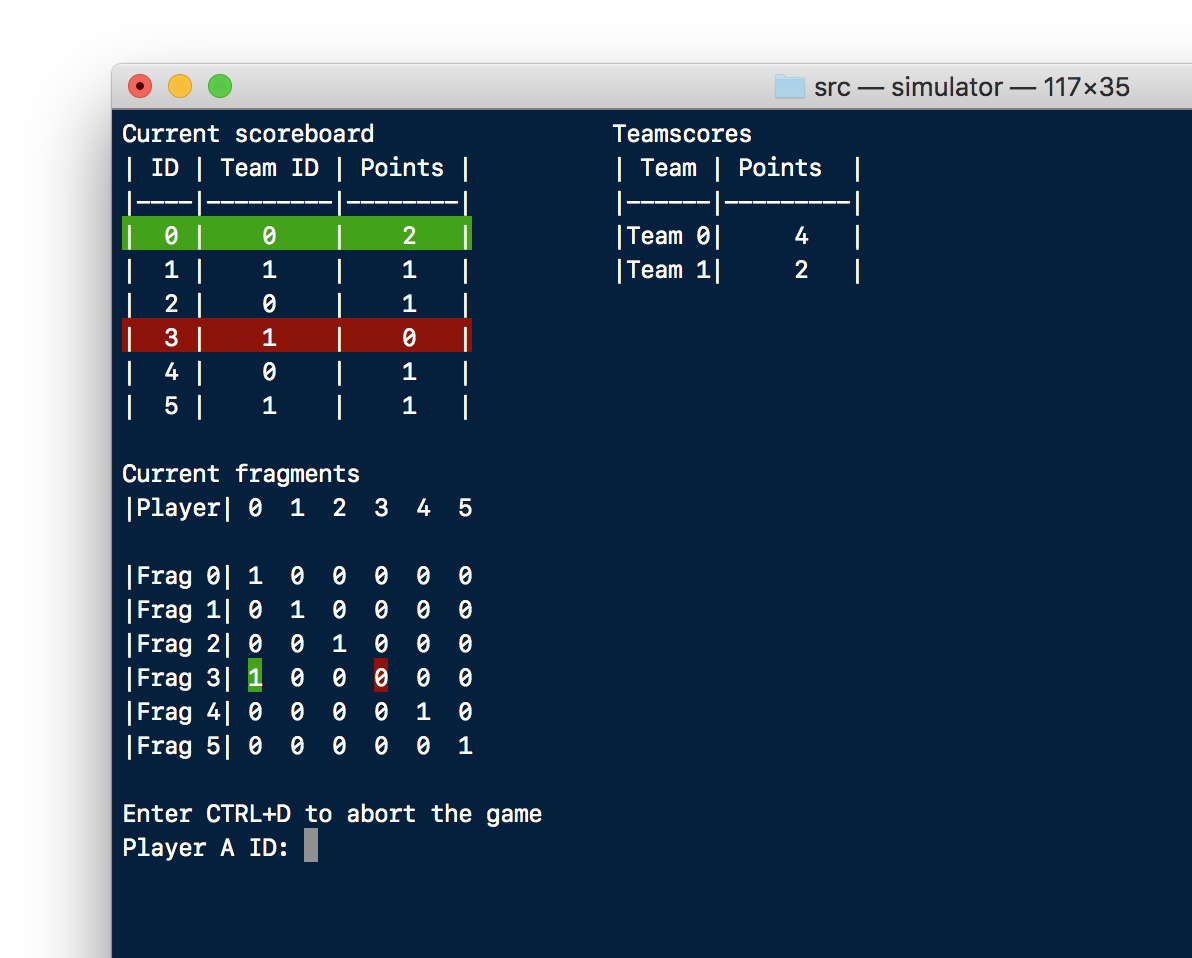
\includegraphics[width=0.7\textwidth,keepaspectratio]{./040-komponenten/030-spielelogik/Simulator.png}
  \caption{Der Simulator}
  \label{fig:simulator}
\end{figure} \\
Ist ein Spiel gestartet, so können Schüsse simuliert werden, indem jeweils die ID eines Schützen und eines Getroffenen eingegeben wird. Anschließend werden die Veränderungen in Punkten und in den Dateifragmenten jedes Spielers sichtbar. Rot hervorgehobene Zahlen stehen dabei für einen Verlust, grün hervorgehobene Zahlen für einen Gewinn, wie in \cref{fig:simulator} zu sehen ist.
Am Ende eines Spiels gibt der Simulator den Gewinner (ein Spieler oder ein ganzes Team) aus. \\
Mehr zu den technischen Aspekten des Simulators ist im \cref{sec:api-zu-services-komponente} zu finden.

\paragraph{Solo Easy}
Bei dem Spielmodus „Solo Easy“ handelt es sich um einen Spielmodus, welcher schnell implementiert werden sollte. Demnach soll der Spielmodus einfach spielbar sein. Der Spielmodus funktioniert wie folgt: \\
Jedem Spieler wird ein Dateifragment zugewiesen. Wird ein Spieler durch einen anderen Spieler getroffen, bekommt der Schütze das ursprüngliche Dateifragment des Getroffenen. Dabei ist zu beachten, dass der getroffene Spieler sein Dateifragment jedoch behält, d.h. Dateifragmente werden bei Treffern somit kopiert. Das Spiel endet, sobald ein Spieler alle existierenden Dateifragmente besitzt.

\paragraph{Solo Advanced}
Der Spielmodus „Solo Advanced“ baut auf dem Spielmodus „Solo Easy“ auf. Der Unterschied hierbei liegt darin, dass bei einem Treffer der getroffene Spieler sein Dateifragment jedoch nicht behält, d.h. Dateifragmente werden nun bei Treffern abgegeben. Das bedeutet also insbesondere, dass Dateifragmente nicht kopiert werden. Ein Dateifragment zählt hierbei wie ein Punkt. \\
Des Weiteren kann der Spielmodus in mehreren Runden gespielt werden, wobei eine Runde durch ein Zeitlimit begrenzt wird. Eine Runde gewinnt derjenige Spieler, welcher die meisten Punkte, also die meisten Dateifragmente am Ende einer Runde besitzt.

\paragraph{Teams Advanced}
Als Variation kann der Spielmodus „Solo Advanced“ auch teambasiert gespielt werden, wobei die Teamzuweisung manuell erfolgt. Gewonnen hat demnach das Team, welches am Ende einer Runde die meisten Punkte hat. Teambeschuss wird hierbei nicht beachtet (ist nicht erlaubt) und führt demnach zu keinem Ereignis (kein Punktabzug o.Ä.).

\paragraph{No Carry No Win}
„No Carry No Win“ ist ein Spielmodus, der ausschließlich teambasiert gespielt wird, wobei die Teamzuweisung manuell erfolgt. Hierbei wird pro Team ein Spieler zufällig ausgewählt, welcher alle Dateifragmente einer begehrten Datei besitzt, der sogenannte „Carry“. Er hat besondere Bedeutung für das BitTorrent-Netzwerk in dem zugrundeliegenden Szenario, denn da er bereits alle Dateifragmente hat, tritt er nur noch als Seed auf und ist für das Netzwerk (sein Team) besonders wichtig. \\
Nun bricht ein Kampf zwischen den Teams aus, ganz im Stile von Lasertag. In diesem Kampf ist folglich das Ziel jedes normalen Spielers (jedes Spielers, der kein Carry ist), seinen Carry zu verteidigen, ihn also im BitTorrent-Netzwerk zu halten, denn sie wollen von ihm in Zukunft auch noch Dateifragmente erhalten können. \\
Jeder normale Spieler besitzt zu Beginn wie üblich ein Dateifragment. Zu beachten ist hierbei, dass in diesem „Kampf“ Dateifragmente nicht kopiert oder übertragen, sondern nur als Leben gewertet werden. Ein Spieler „stirbt“, scheidet also aus einer Runde aus, wenn er kein Dateifragment mehr besitzt. Das bedeutet, dass ein normaler Spieler nach einem Treffer, der Carry jedoch erst nach mehreren Treffern „stirbt“. \\
Der Spielmodus kann in mehreren Runden gespielt werden, wobei eine Runde dann endet, wenn nur noch ein Carry übrig ist. Das Team, dessen Carry zuletzt übrig ist, gewinnt die jeweilige Runde.
Bei diesem Spielmodus wird ebenfalls kein Teambeschuss toleriert.

\paragraph{Share Or No Share}
Der Spielmodus „Share Or No Share“ soll ein fundamentales Prinzip von BitTorrent besonders hervorheben: die Kollaboration. Jeder neue Peer im Netzwerk profitiert zunächst von den bereits angebotenen Dateifragmenten und sollte anschließend, nach Erhalt des ersten Dateifragments, zur Weiterverteilung der entsprechenden Datei beitragen, indem er seinerseits Dateifragmente anderen Peers zur Verfügung stellt. \\
„Share Or No Share“ wird dafür ausschließlich teambasiert gespielt, wobei die Teamzuweisung zufällig erfolgt. Hierbei werden die Spieler in zwei Teams aufgeteilt, ein faires Team und ein unfaires Team. Wieder wird davon ausgegangen, dass jeder Spieler zu Beginn des Spiels bereits ein Dateifragment erhalten hat. Im fairen Team befinden sich „normale“ Peers, die sowohl Dateifragmente von anderen Peers erhalten als auch selbst Dateifragmente zur Verfügung stellen wollen. Im unfairen Team hingegen befinden sich sogenannte „Power-Leecher“, Peers, die also möglichst schnell alle benötigten Dateifragmente bekommen möchten, jedoch keine zur Verfügung stellen wollen. Die Aufteilung in Teams erfolgt bestmöglich in dem Verhältnis 2:1 (faire:unfaire Spieler), weil uns realistisch erscheint, dass es mehr faire als unfaire Peers gibt. \\
Es gewinnt das Team, welches zum Ende des Spiels die meisten Punkte hat. Dabei werden die Punktzahlen nach \cref{tab:share-or-no-share-punkte} vergeben.
\begin{table}
  \centering
  \begin{tabular}{|c|c|c|}\hline
      trifft & fair & unfair \\ \hline
      fair & $+10$ für beide & $+20$ für Schützen \\
       & & $-20$ für Getroffenen \\ \hline
      unfair & $+20$ für Schützen & $+10$ für Schützen \\
       & $-20$ für Getroffenen & $-10$ für Getroffenen \\ \hline
  \end{tabular}
  \caption{Punktevergabe im Spielmodus „Share Or No Share“ \\
           \footnotesize Zu lesen ist die Tabelle in der Form „\emph{\textless Eintrag aus erste Spalte\textgreater\ trifft \textless Eintrag aus erste Zeile\textgreater}“.}
  \label{tab:share-or-no-share-punkte}
\end{table}
Die Motivation für die Punktzahlen ist wie folgt. Offensichtlich werden Punkte nur auf der fairen Seite „erzeugt“. Das soll unterstreichen, dass BitTorrent prinzipiell nur kollaborativ funktioniert, und nur bei fairem Dateiaustausch ein Mehrwert für alle Peers entsteht. Ansonsten spiegeln die Punktzahlen ganz einfach die Motivation der jeweiligen Spieler wider, entsprechend zu treffen oder getroffen zu werden. So wollen faire Spieler beispielsweise, dass alle anderen Peers im Netzwerk auch fair spielen, also Dateifragmente zur Verfügung stellen. Deshalb bekommen sie mehr Punkte, wenn sie einen unfairen Spieler treffen und ihn damit zum Teilen „zwingen“, als wenn sie einen fairen Spieler treffen. Entsprechend sieht es auf der anderen Seite aus. Unfaire Spieler nutzen also gern die fairen Spieler aus und werden damit mit entsprechend mehr Punkten belohnt. Und für Schüsse innerhalb des unfairen Teams gibt es beim getroffenen unfairen Spieler Punktabzug, weil ein unfairer Spieler mit niemandem „teilen“ möchte. \\
Der Spielmodus hat nur eine Runde, wobei das Spiel endet, sobald ein Spieler alle Dateifragmente gesammelt hat. \\

\noindent
Wir haben die Spielmodi nur mit dem Simulator und nicht im Praxiseinsatz, also auf einem echten Spielfeld mit echten Spielern, testen können. Dadurch könnten uns Faktoren, die den Spielverlauf in der Praxis beeinflussen und damit eventuell Anpassungen an den Annahmen und bspw. Punktzahlen der Spielmodi nötig machen würden, völlig unbekannt geblieben sein. Besonders für das Balancing von Parametern wie Punktzahlen und die Zuweisung der initialen Dateifragmente hätte ein automatisches Testen sinnvoll sein können. Andererseits hätten auch bei automatischen Tests Rahmenbedingungen bzw. Testcases festgelegt werden müssen, die ohne Daten aus der Praxis nur schwer realistisch festgelegt hätten werden können.

Alle drei Mitglieder der Spiellogik Gruppe haben Ideen für Spielmodi vorgeschlagen, die gemeinsam diskutiert wurden. Die Spielmodi „Solo Advanced“ und „Teams Advanced“ sind Ideen von David Bachorska. Der Spielmodus „No Carry No Win“ wurde von Dennis Ness und „Share Or No Share“ von Tom Kieseling entwickelt.

\subsubsection{API zu Services Komponente}
\label{sec:api-zu-services-komponente}

Als grundsätzliche Designentscheidung verwendet jeder Spielmodus ein eigenes Lua Skript.
Dies ist sinnvoll, da sich die Spielmodi teils massiv unterscheiden, denn es gibt z.B. je nach
Spielmodus vollkommen verschiedene Start- und Siegbedingungen. Somit muss es
zwischen der Spiellogik und der Services Komponente klar sein, welches Lua Skript bzw. welcher
Spielmodus gerade gespielt wird. Dieses Problem wird gelöst durch die Art und Weise, wie
ein Lua Skript in C++ eingebunden wird.

Denn die API zu der Services Komponente nutzt die von Lua bereitgestellte C++ API. Somit
ist es problemlos möglich, sowohl Funktionen von C++ heraus in den Lua Skripten
aufzurufen, als auch von den Lua Skripten aus C++ Funktionen aufzurufen. Hier wurden
beide Richtungen genutzt und gebraucht, wobei über das gesamte Spiel und auch der
Anzahl der Funktionen hinweggesehen die meisten Aufrufe von den Lua Skripten zu den C++ Funktionen laufen.

Die Entwicklung der API ging stark einher mit der Entwicklung des Simulators, da dieser die
API verwendet. Es war also erforderlich, möglichst schnell eine stabile API zu haben, um mit
der Entwicklung der Spielmodi beginnen zu können. Aufgrund dieser frühen Festlegung
blieb zwar die grundlegende API im Laufe der Entwicklung erhalten, hat aber einige
Erweiterungen erfahren.

Um einen Überblick über die API zu erhalten, werden hier nun die drei Hauptbestandteile,
die die API abdeckt, erläutert: Die Spielinitialisierung, der normale Spielablauf und zum
Schluss das Spielende.
Wie bereits erwähnt, läuft die meiste Kommunikation von den Lua Skripten zu der Services
Komponente. Ausnahmen bilden hier der Start des Spiels, wenn die Zeit einer Runde abläuft
und wenn ein Spieler einen anderen Spieler trifft. Ein Großteil der Funktionen der API
beschäftigt sich mit der Initialisierung des Spiels. Dazu werden eine Reihe von
Spielparametern abgefragt, wie z.B. die Anzahl der Spieler, die Rundendauer oder auch die
Zeit der Unverwundbarkeit eines Spielers. Diese Informationen werden in den
entsprechenden Lua Skripten verarbeitet und weitere Funktionen in C++ werden zur
Dateiverwaltung aufgerufen.
Ein gutes Beispiel dafür ist die Festlegung der Anzahl der Dateifragmente jedes Spielers.
Um diese Aufgabe zu bewältigen wird zunächst über die API die Anzahl der Spieler
abgefragt. Dann wird ebenfalls über die API der C++ Komponente mitgeteilt, wie viele
Dateifragmente jeder Spieler maximal besitzen kann. Anschließend bestimmt das Lua
Skript, welcher Spieler welche Dateifragmente besitzt. Diese Information wird dann
ebenfalls über die API an die C++ Komponente übergeben.

Nachdem die Spielinitialisierung abgeschlossen ist, wird das Spiel von der C++ Komponente
aus gestartet. Von nun an besteht die Hauptaufgabe der API darin, auf das Aufrufen der
\texttt{shootPlayer(source, target)} Funktion zu warten. Sobald ein Schuss von der Hardware
ausgelöst und von der Services Komponente vorverarbeitet wurde, wird diese \texttt{shootPlayer}
Funktion aufgerufen. Diese Funktion ist der Hauptteil eines jeden Lua Skripts, denn hier
wird entschieden, ob der Schuss zulässig war, z.B. ob der Gegner überhaupt verwundbar ist,
aber auch wer wie viel Punkte und/oder Dateifragmente erhält. Deshalb ist diese Funktion
recht komplex und enthält letztendlich die gesamte Logik eines Spielmodus.

Grundsätzlich gibt es zwei Möglichkeiten, wie ein Spiel enden kann und somit auch wie die
API genutzt wird: 1.) Nach einem Abschuss tritt eine beliebige Siegbedingung ein und es
werden entsprechende C++ Funktionen von dem Lua Skript aufgerufen, um das Ende des
Spiel zu signalisieren und die Auswertung des Gewinners zu starten. 2.) Es läuft ein Zeitlimit
ab. In diesem Fall ruft ein Timer aus der C++ Komponente heraus eine spezielle Lua Callback Funktion auf. Diese spezielle Funktion hält dann das Spiel an und ruft weitere Funktionen auf. Diese zweite Variante ist ein gutes Beispiel für eine Erweiterung der API, die sich sehr gut in die bestehende API integrieren lassen hat.

Es stellt sich also die Frage, inwiefern Verbesserungen an der API und allen davon unmittelbar betrofenen Bestandteilen möglich gewesen wären. Letztendlich ist die API sehr umfassend geworden und deckt alle Funktionalitäten ab, die für die Spielmodi notwendig sind. Allerdings verwendet die API auch sehr viele sehr kleinteilige Funktionen, die zu größeren, umfassenderen Funktionen zusammengefasst werden könnten. Dadurch wäre die API übersichtlicher geworden, ohne an Funktionalität und Flexibilität einzubüßen.
Eine weitere Verbesserungsmöglichkeit setzt nicht direkt bei der API an, sondern bei den
Funktionen innerhalb der Lua Skripte. Dort hätte man für eine bessere Übersicht mehr
Funktionen auslagern können und auch von dem Konzept abrücken können, immer nur ein
Skript für einen Spielmodus zu verwenden. Denn dadurch wären die Skripte noch sehr viel
modularer gestaltbar gewesen. Dies alles wäre der Übersicht zugute gekommen und hätte
beim Debugging helfen können.

Die grundsätzliche Entwicklung der API wurde gemeinsam von allen drei Mitgliedern der
Spiellogik Gruppe durchgeführt. Die erste Umsetzung der API in Form des Simulators
geschah durch Dennis Ness. Im Verlaufe des Projekts wurden jedoch eine Reihe von
Erweiterungen von David Bachorska (z.B. Teamhandling) und Tom Kieseling (z.B.
Teamzuweisung von Lua aus) zu der API hinzugefügt. Allerdings gab es auch Erweiterungen
der API, die von Personen der Services Gruppe ausgingen. So hat z.B. Jan Arne Sparka eine Erweiterung zur Ansteuerung der LEDs hinzugefügt.



\section{Zusammenfassung}
\label{sec:zusammenfassung}

In diesem Abschnitt wird erläutert, ob das errichtete System die Anforderungen
erfüllt und an welchen Stellen noch Verbesserungen vorgenommen werden könnten.

\subsection{Auswertung}

Es gibt zwei Sichten darauf, wieviel von der geplanten Architektur umgesetzt wurden: zum einen die
Implentierung der einzelnen Komponenten, zum anderen die Integration derselben.
Um eine technische Machbarkeit der Lösung zu demonstrieren, reicht es aus, mit Unit Tests die
Funktionalität der Einzelkomponenten zu beweisen.
Allerdings war als Endprodukt ein Spiel gefordert, wofür es notwendig ist, dass die Integration
reibungslos funktioniert.
Das heißt, ein beliebiger externer Spieler kann das System verwenden, ohne Kenntnisse über deren
interne Funktionsweise zu haben.

Die einzelnen Komponenten, die geplant waren, wurden alle implementiert und zumindest teilweise
getestet.
Die Spielelogikgruppe konnte mit einem Simulator demonstrieren, dass die einzelnen Spielmodi das
Soll-Verhalten aufweisen und die Hardware-Gruppe konnte mit Hilfe eines Treibers demonstrieren, dass
Infrarotabschüsse an den Services-Client durchgereicht und LED Events korrekt angezeigt werden.
Die Services-Gruppe hat die Funktionalität der Webseite demonstriert, indem sie manuell Einträge in
die Datenbank hinzufügten und bestätigten, dass jene Änderungen auf der Webseite übernommen werden. 
Auch grundlegende Client-Server Kommunikation war möglich.

Die Integration der Komponenten ist unvollständig.
Es lässt sich nachweisen, dass der Server mit LUA kommuniziert.
Allerdings lassen Logs darauf schließen, dass Parameter in der falschen Reihenfolge an LUA
weitergegeben werden.
Die Webseite-zu-Server-Integration über die Datenbank funktioniert für einfache Spielmodi, bei
komplexeren bringen jedoch Deadlocks von Mutex-Objekten den Server zum Absturz.
Es kam außerdem zu diversen Fehlern bei Zugriffen des Servers auf die Datenbank.
Der Services-Server und der Services-Client können sich miteinander verbinden und
Abschussinformationen werden ausgetauscht.
Allerdings führt ein Verbindungsverlust des Clients zurzeit noch dazu, dass der zugehörige Spieler sich 
nicht mehr mit dem Spiel verbinden kann.
Diese Problem machen derzeit einen Neustart der Systemd-Units auf allen Geräten notwendig, wenn ein
neues Spiel gestartet wird.
Die Verbindung der Client/Server-Programme mit Systemd ist noch instabil.
Es dauert teilweise Minuten, bis eine Unit gestoppt werden kann.
Die Hardware-API ist in der Lage, zuverlässig Abschussinformationen an den Services-Client
weiterzugeben.
Allerdings werden derzeit keine LED-Events an die Hardware-API gesendet.
Die Integration der Hardware-API mit der darunter liegenden Hardware und Systemd ist stabil und
verursacht keine Probleme.


\subsection{Ausblick}

Aus dem letzten Abschnitt geht hervor, dass ein Spiel bis zu einem gewissen Punkt demonstriert
werden kann, jedoch ist ein ausgereiftes Spiel noch nicht möglich, von Spaß kann nicht die Rede
sein.
Die geplante Architektur erfüllt jedoch die Aufgabenstellung und sie wurde größtenteils umgesetzt.
Viele der genannten Probleme könnten nach einigen Tagen Bugfixing behoben werden und sobald die
Integration der Komponenten stabil ist kann ein richtiges Spiel gespielt werden.
Ob man dabei auch Spaß hätte bleibt offen, dies lässt sich mit einem Simulator nicht demonstrieren
und wahrscheinlich wären viele weitere Tests notwendig, bis das Produkt ausgereift und tauglich für
die Allgemeinheit wäre.



\end{document}
